\documentclass[12pt]{report}
\usepackage[T1]{fontenc}
%\usepackage{polski}
\usepackage[utf8]{inputenc}
\usepackage{graphicx}
\usepackage{wrapfig}
\usepackage{amsmath,amssymb,amsfonts}
\usepackage{txfonts}
\usepackage{placeins}
\usepackage{listings}
\usepackage{listings-golang} 
\usepackage{pdfpages}
\usepackage{color}
\usepackage{xcolor}
\usepackage{framed}
\usepackage{filecontents}
\usepackage{caption}
\usepackage{adjustbox}
\usepackage{textcomp}

\usepackage[polish]{babel}

\usepackage{caption}
\DeclareCaptionFont{white}{\color{white}}
\DeclareCaptionFormat{listing}{\colorbox{gray}{\parbox{\dimexpr\linewidth-2\fboxsep\relax}{#1#2#3}}}
\captionsetup[lstlisting]{format=listing,labelfont=white,textfont=white}

\let\Oldsection\section
\renewcommand{\section}{\FloatBarrier\Oldsection}

\let\Oldsubsection\subsection
\renewcommand{\subsection}{\FloatBarrier\Oldsubsection}

\let\Oldsubsubsection\subsubsection
\renewcommand{\subsubsection}{\FloatBarrier\Oldsubsubsection}

\renewcommand{\chaptername}{Rozdział}
\renewcommand{\contentsname}{Spis treści}
\renewcommand{\figurename}{Rys.}
\renewcommand{\tablename}{Tab.}
\renewcommand{\listfigurename}{Spis rysunków}
\renewcommand{\listtablename}{Spis tabel}
\renewcommand{\bibname}{Bibliografia}

\pagestyle{headings}

\setlength{\textwidth}{14cm}
\setlength{\textheight}{20cm}

\newtheorem{cloudcomputing}{Chmura obliczeniowa}

\lstset{
%    frame=single,
    breaklines=true,
    backgroundcolor=\color{gray!10},
}

\newcommand\YAMLcolonstyle{\color{red}\mdseries}
\newcommand\YAMLkeystyle{\color{black}\bfseries}
\newcommand\YAMLvaluestyle{\color{blue}\mdseries}

\makeatletter

% here is a macro expanding to the name of the language
% (handy if you decide to change it further down the road)
\newcommand\language@yaml{yaml}

\expandafter\expandafter\expandafter\lstdefinelanguage
\expandafter{\language@yaml}
{
  keywords={true,false,null,y,n},
  keywordstyle=\color{darkgray}\bfseries,
  basicstyle=\YAMLkeystyle,                                 % assuming a key comes first
  sensitive=false,
  comment=[l]{\#},
  morecomment=[s]{/*}{*/},
  commentstyle=\color{purple}\ttfamily,
  stringstyle=\YAMLvaluestyle\ttfamily,
  moredelim=[l][\color{orange}]{\&},
  moredelim=[l][\color{magenta}]{*},
  moredelim=**[il][\YAMLcolonstyle{:}\YAMLvaluestyle]{:},   % switch to value style at :
  morestring=[b]',
  morestring=[b]",
  literate =    {---}{{\ProcessThreeDashes}}3
                {>}{{\textcolor{red}\textgreater}}1     
                {|}{{\textcolor{red}\textbar}}1 
                {\ -\ }{{\mdseries\ -\ }}3,
}

% switch to key style at EOL
\lst@AddToHook{EveryLine}{\ifx\lst@language\language@yaml\YAMLkeystyle\fi}
\makeatother

\newcommand\ProcessThreeDashes{\llap{\color{cyan}\mdseries-{-}-}}

\begin{document}


\includepdf{images/title-page.png}

\tableofcontents    % generuje spis treści ze stronami

\chapter{Wstęp}\label{chap:wstep}
\section{Problematyka i zakres pracy}
Wraz z rozwojem Internetu Rzeczy\footnote{Internet Rzeczy (ang. Internet of Things) - koncepcja inteligentnego zarządzania otoczeniem i wymiany danych przy wykorzystaniu urządzeń codziennego użytku \cite{iot}.} na świecie powstają coraz to nowe urządzenia mające na celu automatyzację działań i ułatwienie życia człowieka. Dzięki ich zdolności do wzajemnej komunikacji, wymiany informacji oraz zdalnego zarządzania zasobami stają się one coraz bardziej popularne, a wręcz wymagane w życiu codziennym coraz większej grupy osób. Sterowanie oświetleniem, radiem czy innymi sprzętami elektronicznymi za pomocą naszego smartfona już nikogo nie dziwi. W wielu przypadkach urządzenia te muszą zbierać bardzo duże ilości danych oraz przesyłać je do centralnego punktu. Powoduje to ogromny wzrost ilości danych, które nie są w stanie zostać obsłużone przez jeden serwer. Powstaje więc potrzeba stworzenia niezawodnych, wydajnych i bezpiecznych systemów o wysokiej dostępności. \\
\indent Technologie wirtualizacji
\footnote{Wirtualizacja (ang. virtualization) - abstrakcja fizycznych zasobów sprzętowych w celu udostępnienia logicznych zasobów. \cite{virtualization}}
powstały w celu realizacji tych wymagań. Wirtualizacja serwerów dawno już wyparła tradycyjne serwery, które zostały zastąpione przez rozwiązania chmurowe. Niezależność sprzętowa, lepsza utylizacja zasobów, większe bezpieczeństwo, łatwa migracja danych i redukcja kosztów to tylko niektóre z wielu zalet wirtualizacji. Właśnie ta niezależność sprzętowa pozwala na coraz lepsze wykorzystanie mikrokontrolerów, których głównymi zaletami są mały koszt i niewielki pobór mocy, a dzięki coraz lepszej optymalizacji systemów i postępującej miniaturyzacji, również rosnąca wydajność. \\
	\indent Obecnie nie trzeba już wydawać ogromnych kwot w celu uruchomienia własnego klastra do zarządzania danymi, czy wyposażenia naszego mieszkania, a nawet biura w inteligentne czujniki i kontrolery. Wystarczą nam w tym celu mikrokontrolery Raspberry Pi, które dzięki systemom typu open source takim jak Kubernetes pozwolą nam na stworzenie w pełni funkcjonalnego klastra. \\
	\indent Proponowanym rozwiązaniem powyższych problemów będzie projekt o nazwie KubePi. Projekt ten skupia się na wirtualizacji opartej o kontenery Dockera
	\footnote{Docker - narzędzie oferujące wirtualizację zasobów opartą o kontenery \cite{docker}.}
zarządzane przez system zarządzania klastrem Kubernetes i ma na celu stworzenie rozproszonego systemu służącego do monitorowania otoczenia. Przykładowy klaster opierać się będzie na dwóch mikrokontrolerach Raspberry Pi. Do pierwszego urządzenia będącego zarazem głównym węzłem klastra podłączone zostaną trzy czujniki: temperatury, wilgotności oraz alkoholu. Jego zadaniem będzie udostęp\-nianie zbieranych informacji. Drugie urządzenie zostanie natomiast wyposażone w wyświetlacz LED, co pozwoli na odczyt i wyświetlanie temperatury raportowanej przez pierwsze urządzenie. Dodatkowo w klastrze zostanie zainstalowana aplikacja webowa
\footnote{Aplikacja webowa (ang. web application) - program pracujący na serwerze, komunikujący się przez sieć komputerową z komputerem użytkownika z wykorzystaniem przeglądarki internetowej \cite{webapp}.}
pozwalająca na zdalny monitoring. W celu lepszego zobrazowania komunikacji między urządzeniami zostanie ona uruchomiona na drugim urządzeniu.

\section{Uzasadnienie wyboru tematu}
W tej części opisane zostaną powody wyboru tematu związanego z systemem monitorowania otoczenia przy użyciu nowoczesnych technologii w oparciu o mikrokontrolery. Głównym powodem jest wykazanie użyteczności systemów chmurowych wysokiej dostępności w oparciu o mikrokontrolery. Wymaga to gwarancji pracy systemu nawet w razie uszkodzenia jednego z węzłów klastra. Drugim powodem jest zbadanie możliwości mikrokontrolerów jako alternatywy dla standardowych systemów chmurowych oraz porównanie wydajności względem ceny przy budowaniu klastra. Ze względu na małe rozmiary i koszt mikrokontrolery takie jak Raspberry Pi mogą służyć jako tania alternatywa do budowy inteligentnego systemu dla naszego domu i nie tylko.

\section{Metoda badawcza}
\begin{enumerate}
\item Studia literaturowe z zakresu chmur obliczeniowych, wirtualizacji oraz mikrokontrolerów. \\ \\
Obecnie dostępne źródła z zakresu chmur obliczeniowych oraz wirtualizacji nie są dobrze sformalizowane. Dostępne są opisy i dokumentacje istniejących systemów, które uwzględniają
w sposób ogólny ich budowę oraz działanie. Znalezione i użyte w tej pracy źródła nie są dostępne w języku polskim, więc muszą być tłumaczone w większości z języka angielskiego.
Jako że nie ma oficjalnych książek dotyczących tematyki chmur obliczeniowych ani wirtualizacji, większość źródeł tu zebranych to źródła elektroniczne, artykuły i dokumentacje. Dostępność książek dotyczących mikrokontrolerów stoi na wyższym poziomie, więc w pracy zostało wykorzystane kilka pozycji poruszających tą tematykę.
\item Analiza wymagań aplikacji uruchamianych w klastrze bazującym na systemie zarządzania klastrem Kubernetes. \\ \\
W związku z tym, że system Kubernetes jest bardzo młody, nie istnieją lepsze źródła o tej tematyce niż oficjalna dokumentacja. Wszelkie wymagane informacje zostały zaczerpnięte z dokumentacji oraz jako, że jest to system otwartoźródłowy, dodatkowym źródłem informacji było oficjalne repozytorium Kubernetesa dostępne na portalu GitHub.
\item Proces projektowania i tworzenia KubePi. \\ \\
W oparciu o zebrane informacje i wymagania aplikacji uruchamianych w klastrze Kubernetesa zostanie stworzony rozproszony system oparty o mikrokontrolery Raspberry Pi. Jego zadaniem będzie monitorowanie otoczenia w oparciu o stworzone aplikacje, co pozwoli na rozwiązanie problemów zidentyfikowanych w procesie analizy.
\item Wnioski dotyczące stworzonego systemu do monitorowania otoczenia. \\ \\
Metoda ta służy do wyciągnięcia wniosków na temat stworzonego systemu oraz aplikacji. Na podstawie działania systemu wyciągnięte zostaną odpowiednie wnioski dotyczące sposobu rozwiązania przedstawionych w pracy problemów oraz projektu KubePi. Wszystko to pozwoli stwierdzić czy proponowane rozwiązanie spełnia postawione w pracy założenia.

\end{enumerate}

\clearpage

\section{Przegląd literatury w dziedzinie}
\subsubsection{Źródła z zakresu języka Go i biblioteki ReactJS}
	\indent Głównym źródłem z zakresu języka Go była dokumentacja. Przydatnymi pozycjami były opisy struktur i kanałów zawarte w sekcji \textit{Effective Go} \cite{effectiveGo} oraz wskazówki dotyczące kompilacji dostępne w sekcji \textit{Compiling Go} \cite{compileGo}. W przypadku biblioteki ReactJS również została wykorzystana głównie dokumentacja dostępna na stronie głównej projektu \cite{reactJSDoc}.
\subsubsection{Źródła z zakresu Internetu Rzeczy}
	\indent W przypadku tematyki z zakresu Internetu Rzeczy wartościową pozycją okazała się książka \textit{The Internet of Things: Enabling Technologies, Platforms, and Use Cases} \cite{iot} oraz w dużej mierze własne doświadczenie zdobyte przy pracy z technologiami chmurowymi.
\subsubsection{Źródła z zakresu chmur obliczeniowych}
	\indent Ze względu na dużą popularność tematu chmur obliczeniowych wybór książek z tej dziedziny jest dość duży. Wymagane było przedstawienie zagadnień teoretycznych w przystępny i prosty sposób w czym pomogła pozycja \textit{Cloud Computing: Concepts, Technology \& Architecture} \cite{cloud}.
\subsubsection{Źródła z zakresu wirtualizacji}
	\indent Wirtualizacja jako jedno z podstawowych zagadnień poruszanych w pracy musiało zostać dobrze wyjaśnione. Tutaj również dużą rolę odniosło własne doświadczenie, wraz z wykorzystaniem książek \textit{Virtualization Essentials} \cite{virtualization} oraz \textit{Docker in Action} \cite{docker}.
\subsubsection{Źródła z zakresu Kubernetesa}
	\indent Kubernetes jako względnie nowy system nie posiada wielu formalnych źródeł, z których można pozyskać informacje. W tym wypadku wymagane było posiłkowanie się głównie przy opisie dokumentacją \cite{kubernetes}.
\subsubsection{Źródła z zakresu mikrokontrolerów}
	\indent W tym wypadku wybór źródeł był bardzo duży i szczegółowy. Ze względu na dobre opinie i dużą popularność wybór padł na książkę autorstwa \textit{Timothy Shorta} pod tytułem \textit{Raspberry Pi 3: Beginner to Pro – Step by Step Guide} \cite{raspberry}, która w przystępny sposób wraz z przykładami opisuje mikrokontrolery Raspberry Pi oraz interfejsy komunikacyjne użyte przy tworzeniu aplikacji. Dodatkowym źródłem informacji była dokumentacja użytych czujników \cite{ds18b20Doc} \cite{max7219Doc} \cite{dht11Doc}  \cite{mq3Doc}.
	
\section{Układ pracy}
Celem pracy jest zaproponowanie architektury i sprawdzenie w działaniu rozproszonego systemu wysokiej dostępności służącego do monitorowania otoczenia. \\
\indent Rozdział pierwszy zawiera szczegółowy opis problemu. Zostają w nim przedstawione różne problemy związane z wydajnością oraz bezpieczeństwem tradycyjnych rozwiązań, wraz z opisem metod badawczych użytych do analizy tematu. Podsumowane zostają również główne założenia i cele pracy. Na koniec przeprowadzony zostaje przegląd literatury związanej z tematem, z naciskiem na kluczowe zagadnienia dotyczące wirtualizacji, rozwiązań chmurowych oraz mikrokontrolerów opartych na architekturze ARM, wraz z krótkim opisem użytych źródeł. \\
\indent W rozdziale drugim przybliżona zostaje tematyka systemów zarządzania klastrami pod kątem ich wymagań, bezpieczeństwa oraz komunikacji sieciowej. Kolejnym krokiem jest dokładniejsze zapoznanie się z wirtualizacją, a konkretniej wirtualizacją opartą o kontenery Dockera, co pozwoli lepiej zrozumieć ideę pracy. Następnie pokrótce przedstawione zostają tematyki związane z mikrokontrolerami oraz Internetem Rzeczy. \\
\indent Kolejny rozdział opisuję fazę projektowania i implementacji projektu KubePi. Spisane zostają wymagania funkcjonalne aplikacji, a także ograniczenia projektowe. Wymienione i opisane zostają użyte technologie. Opisany zostaje proces konfiguracji urządzeń, sieci oraz systemu. Następnie wskazane zostają kluczowe punkty aplikacji wraz z kodem źródłowym i opisem. W kolejnym kroku przechodzimy do fazy testów stworzonych aplikacji jak i całego systemu. \\
\indent W podsumowaniu pracy opisane zostają słabe i mocne strony przedstawionego rozwiązania. Na podstawie uzyskanych wyników następuje ocena możliwości i przydatności zaproponowanego rozwiązania. Na końcu omówione zostają możliwe perspektywy rozwoju projektu.

\chapter{Podstawy teoretyczne}\label{chap:background}
Użyte koncepcje i terminy używane w dalszej części pracy muszą zostać wyjaśnione w celu lepszego zrozumienia opisywanej problematyki. W kolejnych sekcjach zostają objaśnione podstawowe pojęcia związane z Internetem Rzeczy, przetwarzaniem danych w klastrze, tematyką wirtualizacji, rozproszonych systemów chmurowych oraz mikrokontrolerów. Następuje przedstawienie narzędzi do tworzenia, wdrażania i uruchamiania aplikacji rozproszonych w oparciu o kontenery aplikacji Docker. Następnie opisane zostaną systemy zarządzania kontenerami w klastrze takie jak Kubernetes czy trochę mniej zaawansowany Docker Swarm. Na koniec opisany zostanie system oparty o kontenery Dockera, który przenosi zalety kontenerów do Internetu Rzeczy, czyli Resin.io oraz kontroler Raspberry Pi wraz z interfejsami komunikacyjnymi użytymi przy tworzeniu tej pracy.

\section{Internet Rzeczy}
Internet Rzeczy zyskuje na popularności, głównie za sprawą swojego podejścia do komunikacji. Głównym założeniem jest umożliwienie urządzeniom oraz zwykłym przedmiotom codziennego użytku wzajemnej interakcji ze sobą jak i z użytkownikiem. Celem natomiast jest stworzenie inteligentnych urządzeń w celu zminimalizowania i jak największego uproszczenia interakcji użytkownika z takimi urządzeniami. Zaczynając od prostych czujników i wyświetlaczy a kończąc na autonomicznych pojazdach, budynkach czy całych miastach zarządzanych przez mikrokontrolery. 

\begin{figure}[h]
	\centering
	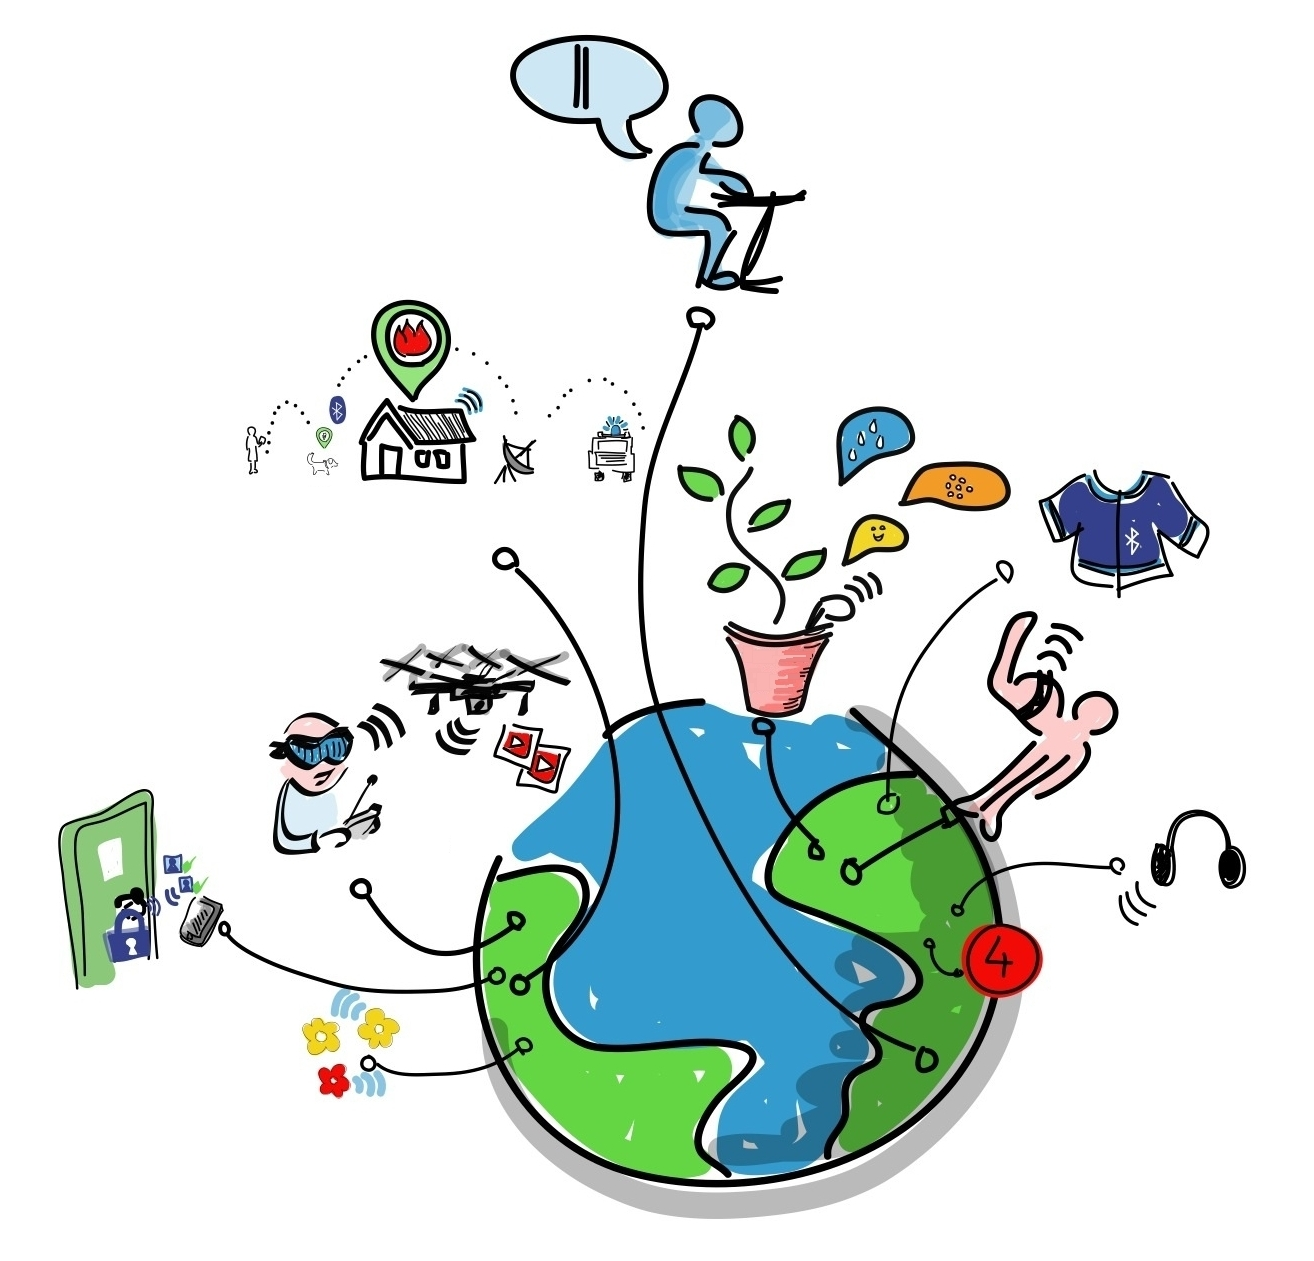
\includegraphics[width=0.6\textwidth]{images/iot.jpg}
	\caption{Przedstawienie Internetu Rzeczy w ujęciu graficznym \cite{iotImg}.}
\end{figure}

\subsection{Obszary zastosowań}
Należy zaznaczyć, że systemy realizacji Internetu Rzeczy są w zasadzie ograniczone tylko przez naszą wyobraźnię, a obejmują one między innymi:
\begin{itemize}
	\item Inteligentne domy i budynki \\ \\
	Interfejsy nowej generacji pozwolą nam nie martwić się o to czy zgasiliśmy światło, albo czy zamknęliśmy drzwi. System sam wykryje czy jesteśmy w domu lub pokoju i zrobi to za nas. Możliwość zarządzania urządzeniami codziennego użytku znacznie podwyższy nasz komfort i bezpieczeństwo.
	\item Inteligentne miasta \\ \\
	Zaawansowane systemy pozwolą zoptymalizować infrastrukturę miejską. Dzię\-ki zbieranym danym system sterowania ruchem sam dostosuje się do panujących warunków i pozwoli na rozładowanie ruchu w mieście. Sieć czujników może zostać użyta do wykrywania przestępstw czy sterowania oświetleniem w mieście.
	\item Inteligentne przedsiębiorstwa i przemysł \\ \\
	Obecnie możemy doświadczyć dużych zmian w przedsiębiorstwach, które wykorzystują Internet Rzeczy w celu zarządzania całym łańcuchem produkcji i dostaw. Inteligentne maszyny same wiedzą w jakim są stanie i mogą reagować odpowiednio wcześnie w celu wymiany podzespołów czy przeprowadzenia konserwacji. Dla klienta natomiast dużym udogodnieniem mogą być zamówienia dostarczane przez drony, które są już testowane przez niektóre duże firmy takie jak Amazon czy UPS.
	\item Monitorowanie otoczenia i zagrożeń \\ \\
	Rozległe sieci czujników już teraz pozwalają na całodobowe monitorowanie temperatury, opadów, wiatru, poziomu rzek, itp. Zebrane dane są przetwarzane i służą do wykrywania anomalii i przewidywania zdarzeń, które mogą zagrażać ludziom. W efekcie zwiększają one nasze ogólne bezpieczeństwo.
\end{itemize}

\section{Chmury Obliczeniowe}
Chmury obliczeniowe stają się coraz ważniejszym elementem Internetu Rzeczy. Dostarczają one swoje zasoby i usługi przy użyciu internetu. Słowo chmura opisuje sposób przetwarzania danych, który oderwany jest od naszego systemu, a przeprowadzany jest na zdalnych serwerach. \\
\indent W szerszym ujęciu natomiast chmura jest centrum danych, w którym poszczególne węzły są wirtualizowane przy użyciu wirtualnych maszyn. Głównym powodem używania chmur obliczeniowych jest rozwiązywanie złożonych problemów oraz analiza dużych ilości danych. Wszystkie dane mogą być łatwo udostępniane innym osobom, a dostęp gwarantowany z każdego zakątka świata \cite{cloud}. \\ \\
Bardziej formalna definicja chmur obliczeniowych przedstawia się następująco.
\begin{cloudcomputing}
Dostarczanie usług obliczeniowych, serwerów, magazynu, baz danych, sieci, oprogramowania analiz, itd. za pośrednictwem internetu. Firmy oferujące te usługi obliczeniowe są nazywane dostawcami chmury i zazwyczaj pobie\-rają opłaty za usługi chmury obliczeniowej w zależności od użycia, podobnie jak dostawcy energii elektrycznej lub wody \cite{cloudComputing}.
\end{cloudcomputing}

\subsection{Architektura}
W związku z szybkim rozwojem chmur obliczeniowych, zostały one podzielone na trzy główne modele usług w celu utylizacji mocy obliczeniowej dla konkretnych potrzeb użytkowników. Modele te zostały zilustrowane na poniższym obrazku obrazującym architekturę chmur obliczeniowych. Architektura ta uwzględnia następujące podziały:

\begin{itemize}
\item Infrastruktura jako serwis (z ang. Infrastracture-as-a-Service) --- znana również pod nazwą hardware-as-a-service. Jest najprostszą odmianą usługi chmu\-ry obliczeniowej i pozwala na zdalny dostęp do zasobów sprzętowych. Dostarcza moc obliczeniową, przestrzeń dyskową i zasoby sieciowe. Jednym z najbardziej znanych dostawców takich usług jest Amazon Elastic Compute Cloud.
\item Platforma jako serwis (z ang. Platform-as-a-Service) --- usługa ta oferuje przede wszystkim środowisko deweloperskie oraz zbiór aplikacji, które mogą być używane do tworzenia i uruchamiania własnych aplikacji. Dostarcza bazy danych, serwery webowe, system operacyjny, środowisko uruchomieniowe, przestrzeń dyskową i wiele innych zasobów. Głównymi dostawcami tych usług są obecnie Microsoft Azure oraz Google App Engine.
\item Oprogramowanie jako serwis (z ang. Software-as-a-Service) --- ostatni z modeli usług chmury obliczeniowej, który oferuje przechowywanie i uruchomienie aplikacji klienta na własnych serwerach oraz udostępnienie jej użytkownikom przez internet. Pozwala to na wyeliminowanie potrzeby instalacji oraz uruchamiania aplikacji na komputerze klienta. W efekcie to dostawca usług ma obowiązek zapewnienia ciągłości działania naszej aplikacji. Najbardziej znane usługi SaaS to np. Google Docs czy Google Apps.
\end{itemize}

\begin{figure}[h]
	\centering
	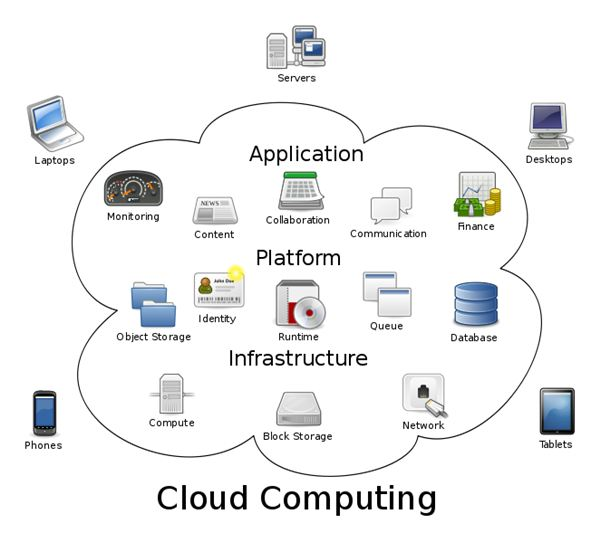
\includegraphics[width=1\textwidth]{images/cloudarchitecture.jpg}
	\caption{Architektura chmur obliczeniowych \cite{cloudArchImg}.}
\end{figure}

\section{Wirtualizacja}
Ze względu na gwałtowny rozwój internetu, zapotrzebowanie na zasoby sprzętowe również wzrasta. Utylizacja i optymalne wykorzystanie zasobów zaczęły odgrywać kluczową rolę. Uruchamianie i zapewnienie ciągłości działania dużym aplikacjom sieciowym stworzyło potrzebę jak najlepszego zarządzania zasobami w celu maksymalnego wykorzystania dostępnych zasobów. Jednym z rozwiązań tych problemów jest właśnie wirtualizacja, czyli stworzenie wirtualnego środowiska zbudowanego w oparciu o infrastrukturę sieciową i dostarczenie go użytkownikom końcowym. \\
\indent Wirtualizacja to tak na prawdę oddzielenie dostępnych zasobów od fizycznego sprzętu. Pozwala to uruchomić wiele systemów na tej samej platformie sprzętowej i systemowej w celu uzyskania jak najlepszej wydajności oraz utylizacji zasobów. Przy użyciu jednej platformy sprzętowej można dostarczyć usługi wielu użytkownikom końcowym. Dwoma najbardziej znanymi podejściami do wirtualizacji są: wirtualizacja oparta o nadzorcę oraz o kontenery. Zostaną one opisane w następnych sekcjach.

\subsection{Wirtualizacja oparta o nadzorcę}
Podejście to w ciągu ostatniej dekady było szeroko używane do tworzenia środowisk wirtualnych dla dużych systemów obliczeniowych. Nadzorca znany również jako monitor wirtualnej maszyny jest oprogramowaniem, które ma za zadanie tworzenie, monitorowanie wirtualnych środowisk oraz przydzielanie im zasobów. Przykładem może być uruchomienie systemu operacyjnego Windows jako maszyny wirtualnej na systemie operacyjnym Linux. \\
\indent Dodatkowo wirtualizacja dostarcza nam niezależne środowisko, które może służyć do uruchamiania aplikacji w izolowanym środowisku bez ingerencji w inne aplikacje. Nadzorców możemy podzielić na dwa typy, które zostały zilustrowane na poniższym rysunku:

\begin{itemize}
\item Native/Bare metal hypervisor --- ten nadzorca działa bezpośrednio na poziomie sprzętu. Dzięki pełnej kontroli nad sprzętem, może kontrolować i monitorować uruchomione systemy operacyjne, które działają poziom wyżej niż nadzorca. Popularnymi przykładami takich nadzorców są: Oracle VM, Microsoft Hyper-V czy VMWare ESX.
\item Host based hypervisor --- ten nadzorca działa jako program uruchomiony na danym systemie operacyjnym (hoście). Pełni on rolę emulatora i izoluje wirtualne systemy operacyjne od sprzętu jak i od hosta, czyli działa dwa poziomy ponad sprzętem. Popularnymi przykładami takich nadzorców są: VirtualBox, VMWare Workstation, KVM.
\end{itemize}

\begin{figure}[h]
	\centering
	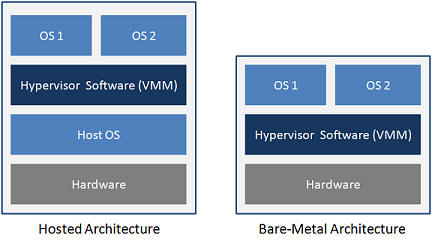
\includegraphics[width=0.9\textwidth]{images/virtualizationArch.png}
	\caption{Architektura wirtualizacji opartej o nadzorcę \cite{hypervisorArchImg}.}
\end{figure}

\subsubsection{Właściwości nadzorcy}
Według książki \textit{Virtualization Essentials} \cite{virtualization} nadzorcy wyróżniają się następującymi właściwościami:
\begin{enumerate}
\item Transparentność --- pozwala uruchamiać oprogramowanie na maszynie wirtualnej bez żadnych modyfikacji i niezależnie od sprzętu oraz umożliwia dzielenie zasobów sprzętowych przez wiele maszyn wirtualnych.
\item Izolacja --- umożliwia nadzorcy tworzenie i uruchamianie niezależnych, odizolowanych od siebie środowisk wirtualnych w obrębie jednego fizycznego systemu. Główną zaletą jest zapobieganie oddziaływania błędów aplikacji na inne aplikacje uruchomione w innych środowiskach wirtualnych.
\item Enkapsulacja --- zapewnia elastyczność i bezpieczeństwo aplikacji uruchomionych w środowisku wirtualnym poprzez zamknięcie systemu w obrębie wirtualnego dysku twardego. Dzięki temu instalacja i tworzenie kopii zapasowych maszyn wirtualnych sprowadza się do kopiowania plików.
\item Prostota zarządzania --- wbudowane opcje nadzorcy do zamykania, restartowania, uruchamiania, usypiania, dodawania oraz usuwania wirtualnych maszyn umożliwiają łatwe zarządzanie wieloma maszynami wirtualnymi.
\end{enumerate}

\subsection{Wirtualizacja oparta o kontenery}
Wirtualizacja oparta o kontenery jest mniej wymagającym w kontekście zasobów podejściem do wirtualizacji. Operuje ona na poziomie systemu operacyjnego i tworzy środowiska wirtualne jako procesy systemowe, co pozwala na dzielenie zasobów sprzętowych z systemem operacyjnym. Wprowadza ona pewien poziom abstrakcji, w którym jądro systemu jest dzielone pomiędzy kontenery i umożliwia uruchamianie więcej niż jednego procesu w obrębie każdego kontenera. Dzięki takiemu rozwiązaniu nie ma potrzeby uruchamiania pełnego systemu operacyjnego odizolowanego od systemu operacyjnego hosta. Przekłada się to bezpośrednio na oszczędność zużycia pamięci, czasu procesora i przestrzeni dyskowej. \\
\indent Na poniższym rysunku możemy zobaczyć trzy kontenery uruchomione w systemie operacyjnym. Zasoby sprzętowe dzielone są pomiędzy nadrzędny system operacyjny oraz systemy operacyjne gości (kontenery). Zaletą tego typu wirtualizacji jest możliwość uruchomienia dużej ilości kontenerów w obrębie jednego systemu operacyjnego. Ma to również swoje wady, a mianowicie nie możemy przykładowo uruchomić systemu operacyjnego Windows jako kontener aplikacji na hoście z systemem operacyjnym Linux. Dodatkowo w porównaniu ze standardowymi nadzorcami kontenery nie gwarantują odpowiedniej izolacji zasobów, co może mieć wpływ na bezpieczeństwo. Funkcje wirtualizacji przy użyciu kontenerów wykorzystują dwie podstawowe właściwości jądra systemu: grupy kontrolne(cgroups) oraz przestrzenie nazw(namespaces).

\begin{figure}[h]
	\centering
	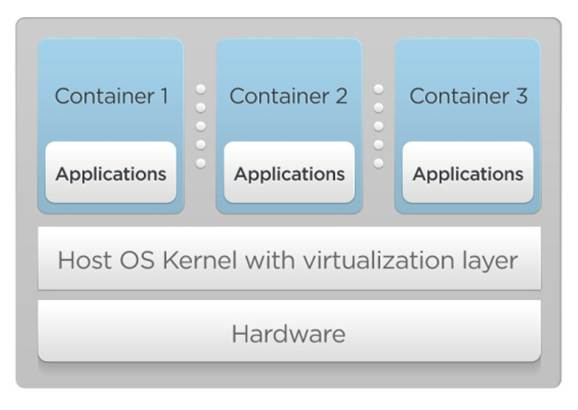
\includegraphics[width=0.8\textwidth]{images/containerArch.jpg}
	\caption{Architektura wirtualizacji opartej o kontenery \cite{hypervisorArchImg}.}
\end{figure}

\subsubsection{Grupy kontrolne}
Grupy kontrolne to jedna z głównych funkcji jądra systemu, która pozwala użytkownikom alokować oraz ograniczać zasoby pomiędzy grupami procesów. Zasoby te to między innymi czas procesora, pamięć systemowa, przestrzeń dyskowa czy wykorzystanie sieci. Grupy kontrolne umożliwiają również sprawne zarządzanie zasobami przeznaczonymi dla kontenerów i działających w nich aplikacji. Przykładowo jeśli aplikacja tworzy dwa procesy z odrębnymi zasobami, może być rozdzielona na dwie grupy kontrolne z różnymi limitami użycia zasobów. Dodatkowo dzięki użyciu grup kontrolnych można w łatwy sposób monitorować i odmawiać lub przyznawać zasoby odpowiednim procesom. Możliwa jest również dynamiczna konfiguracja w trakcie działania systemu. Dzięki temu administrator może w łatwy sposób kontrolować zarządzanie zasobami w systemie \cite{linux}. 

\subsubsection{Przestrzenie nazw}
Przestrzenie nazw to kolejna ważna funkcjonalność dostępna w jądrze systemu, która pozwala na izolacje procesów wewnątrz kontenerów. Gwarantuje ona każdemu procesowi dedykowaną przestrzeń, w której może on działać, bez ingerencji w procesy uruchomione w innych przestrzeniach nazw. Dodatkowo zapewnia izolację środowiska uruchomieniowego procesów \cite{linux}. Obecnie w systemach Linux możemy znaleźć sześć domyślnych przestrzeni nazw:
\begin{itemize}
\item zamontowanych systemów plików (mnt) --- zawiera drzewo katalogów z zamontowanymi systemami plików. Podstawowy system plików jest montowany w korzeniu drzewa w czasie uruchamiania systemu. Utworzenie osobnej przestrzeni nazw systemu plików dla grupy procesów umożliwia zamontowania sytemu plików, który będzie widoczny tylko dla tej grupy procesów. 

\item stacji roboczej i domeny (uts) --- przechowuje aktualną nazwę stacji roboczej oraz nazwę domeny, do której należy stacja robocza. Utworzenie osobnej przestrzeni nazw UTS umożliwia zmianę tych parametrów dla poszczególnej grupy procesów.

\item identyfikatorów procesów (pid) --- umożliwia istnienie wielu procesów w różnych przestrzeniach nazw z tym samym identyfikatorem procesu. Użyteczna przy przenoszeniu grupy procesów między maszynami bez zmiany ich identyfikatorów.

\item obiektów IPC (ipc) --- pozwala na tworzenie systemowych obiektów do komunikacji między procesami, widocznych tylko dla grupy procesów, które współdzielą daną przestrzeń nazw IPC.

\item użytkowników (user) --- pozwala na odizolowanie procesów bazując na identyfikatorze użytkownika i grupy, która uruchomiła dany proces. Dzięki temu dany proces może być uruchomiony z przywilejami administratora w konkretnej przestrzeni nazw, natomiast w innych działać jako proces z prawami zwykłego użytkownika.

\item zasobów sieciowych (net) --- pozwala na odizolowanie podsystemu sieciowego dla grupy procesów. Dzięki temu grupa procesów może konfigurować urządzenia sieciowe oraz nawiązywać połączenia niezależnie od reszty systemu. Taka grupa posiada własne urządzenia sieciowe, adresy IP, trasy, itp.
\end{itemize}

\subsubsection{Właściwości kontenerów}
Możemy wyróżnić cztery właściwości kontenerów, które sprawiają, że są one atrakcyjne dla użytkowników:

\begin{enumerate}
\item Przenośność --- kontenery mogą działać na wielu różnych środowiskach i nie wymagają dodatkowych kroków w celu dostosowania systemu operacyjnego. Dodatkowo można uruchamiać wiele aplikacji w obrębie jednego kontenera, a następnie uruchamiać je na różnych środowiskach.

\item Szybkość tworzenia --- kontenery są łatwe i szybkie w budowie. W porównaniu z tworzeniem standardowej maszyny wirtualnej ich budowa i start zajmują sekundy, a nie minuty. Dzięki temu administratorzy mogą w łatwy sposób uruchamiać kontenery w środowisku produkcyjnym. Dodatkowo skracają czas potrzebny na stworzenie aplikacji uruchamianej w kontenerze. W łatwy sposób pozwalają na dzielenie się aplikacjami z zespołem i testowanie w różnych środowiskach.

\item Skalowalność --- tworzenie i instalacja kontenerów na dowolnym systemie czy w chmurze obliczeniowej są bardzo proste. Dużym plusem jest również skalowalność kontenerów. W prosty sposób możemy zautomatyzować tworzenie czy usuwanie kontenerów bazując na aktualnym zużyciu zasobów sprzętowych. Dzięki temu idealnie nadają się one do instalacji w chmurze.

\item Elastyczność --- przy użyciu kontenerów możemy w prosty sposób uruchomić dużą liczbę aplikacji na pojedynczym systemie operacyjnym. Biorąc pod uwagę, że nie uruchamiają one pełnego systemu operacyjnego, możemy w łatwy i wydajny sposób zarządzać wieloma aplikacjami. 
\end{enumerate}

\subsection{Docker}
Docker jest jednym z najpopularniejszych narzędzi bazujących na wirtualizacji opartej o kontenery. Został on po raz pierwszy przedstawiony przez Solomona Hykesa, 15 marca 2013 roku. W tamtym czasie niewiele, bo około 40 osób uzyskało szansę poznania tego narzędzia. \\
\indent Docker jest narzędziem które w łatwy sposób pozwala na tworzenie i dystrybucję aplikacji na różne środowiska. Dodatkowo umożliwia proste skalowanie i konfigura\-cję naszych aplikacji. Pozwala w znaczący sposób skrócić proces tworzenia i testowania oprogramowania oraz natywnie korzysta z dwóch opisanych wcześniej funkcji jądra systemu, a mianowicie grup kontrolnych i przestrzeni nazw. Ważne jest również to, że Docker pozwala uruchomić niemal każdą aplikację bezpiecznie w kontenerze, dostarczając izolacjęi bezpieczeństwo na poziomie systemu. Pozwala to uruchamiać wiele kontenerów jednocześnie bez obaw, że będą one oddziaływały na siebie w jakikolwiek szkodliwy sposób. Wystarczy jedynie minimalny system operacji ze zgodną wersją jądra systemu oraz plik wykonalny Dockera. \\
\indent W związku z tym, że aplikacje zostają uruchomione w izolowanym środowisku, Docker udostępnia narzędzia dla ułatwienia budowy, uruchamiania i zarządzania kontenerami. Oprócz możliwości uruchomienia go na lokalnym komputerze, istnieje również szereg dostawców usług, którzy wspierają kontenery Dockera, np. Google Cloud Platform, Microsoft Azure, Amazon EC2. Istnieje również platforma o nazwie Resin.io, która oferuje wsparcie systemów opartych na Dockerze dla urządzeń z zakresu Internetu Rzeczy, jednak dokładniej zapoznamy się z nią w sekcji~\ref{subsect:resin}.

\subsubsection{Cele Dockera}
Głównymi celami Dockera sa:
\begin{itemize}
\item Dostarczenie łatwego sposobu modelowania złożonych systemów wymagają\-cych wielu współpracujących aplikacji. Dzięki użytym mechanizmom jest on bardzo szybki i umożliwia łatwe dostosowanie do własnych potrzeb. Dodatkowo uruchamianie kontenerów aplikacji zajmuje w większości przypadków niespełna sekundę oraz nie wymaga uruchamiania nadzorców i zarządza naszymi zasobami systemowymi w bardziej optymalny sposób.

\item Usprawnienie cyklu produkcji poprzez jego przyspieszenie i bardziej efektywne zarządzanie zasobami. Głównym celem jest tu redukcja czasu potrzebnego na tworzenie i testowanie oprogramowania, a zapewnione jest to głównie dzięki zapewnieniu możliwości uruchamiania tej samej aplikacji w wielu środowiskach bez dodatkowych zmian.

\item Spójność aplikacji uruchamianych na różnych środowiskach, dzięki użyciu wirtualizacji opartej o kontenery. Zapewnia to, że nasza aplikacja będzie zachowywała się tak samo niezależnie od tego na jakim systemie uruchamiany jest kontener z nią.
\end{itemize}

\subsubsection{Architektura Dockera}
Docker bazuje na modelu klient-serwer. Klient Dockera komunikuje się z demonem\footnote{Demon (ang. daemon) - program lub proces, wykonywany wewnątrz środowiska systemu operacyjnego, bez konieczności interakcji z użytkownikiem \cite{linux}.}, który odpowiada za tworzenie, uruchamianie oraz dystrybucję kontenerów. Zazwyczaj oba te komponenty uruchamiane są na tej samej maszynie, jednak możliwe jest uruchomienie demona na zdalnej maszynie i podłączenie się do niej za pomocą aplikacji klienckiej. Architektura została pokazana na poniższym rysunku. Każdy z komponentów ma określone zadania, które zostaną opisane poniżej.

\begin{figure}[h]
	\centering
	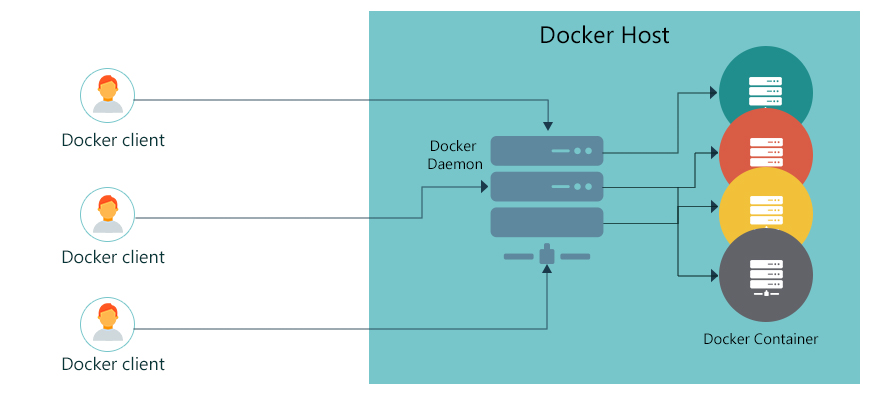
\includegraphics[width=1\textwidth]{images/dockerArch.jpg}
	\caption{Architektura dockera \cite{dockerArchImg}.}
\end{figure}

\subsubsection{Demon Dockera}
Głównym zadanie tego komponentu jest zarządzanie działającymi kontenerami. Jak widać na powyższym rysunku demon uruchomiony jest na systemie, na którym działają kontenery. Klient natomiast używany jest w celu komunikacji z demonem, ponieważ użytkownik nie może bezpośrednio się z nim komunikować.

\subsubsection{Klient Dockera}
Aplikacja kliencka Dockera jest, interfejsem uruchamianym z poziomu konsoli. Służy ona do komunikacji z procesem demona. Użytkownik poprzez odpowiednie komendy klienta może pośrednio komunikować się z demonem.

\subsubsection{Obrazy Dockera}
Obrazy są podstawowym źródłem służącym do tworzenia kontenerów. W pewnym sensie są one kodem źródłowym kontenerów. Obrazy można budować samemu praktycznie od zera lub użyć już istniejących obrazów dostępnych na platformach takich jak DockerHub\footnote{DockerHub - strona będąca oficjalnym darmowym repozytorium aplikacji Dockera \cite{dockerhub}.}. Umożliwiają one prostą konfigurację oraz tworzenie nowych obrazów. Dodatkowo dzięki dostępności darmowych repozytoriów można łatwo i szybko się nimi dzielić. \\
\indent Obrazy złożone są z wielu warstw instrukcji. Przykładowo, użytkownik może zdefiniować, aby przy tworzeniu obrazu uruchomiona została odpowiednia komenda systemowa, skopiowany folder czy ściągnięte dodatkowe zależności potrzebne do uruchomienia aplikacji. Następnie wszystkie warstwy są łączone w celu stworzenia obrazu. Dzięki takiemu podejściu do tworzenia obrazów, jeśli aktualizujemy tylko naszą aplikację, nie wymaga to przebudowy innych warstw, a jedynie aktualizacji warstwy zawierającej naszą aplikację.

\subsubsection{Rejestr Dockera}
Rejestry używane są do przechowywania stworzonych obrazów. Mogą być one prywatne lub publiczne. Publicznym rejestrem jest przykładowo wspomniany wcześniej DockerHub. Jest to jedna z najpopularniejszych platform służąca do przechowywania obrazów Dockera. Możemy z łatwością znaleźć obraz serwera dla naszej aplikacji webowej, bazę danych czy nawet cały system operacyjny. Jeśli nie chcemy natomiast dzielić się naszymi obrazami z innymi, możemy z łatwością skorzystać z prywatnych rejestrów, które również mogą być uruchamiane jako kontenery Dockera i udostępniać je tylko w obrębie naszej organizacji.

\subsubsection{Kontenery}
Jak już wcześniej wspomniano, kontenery tworzone są przy użyciu obrazów, które mogą zawierać również aplikacje i różne serwisy. Uruchamiają aplikacje w odizolowanym środowisku zawierającym wszystkie zależności wymagane do ich działania. 

\section{Systemy zarządzania kontenerami}
Jedną z największych zalet kontenerów jest możliwość zarządzania nimi jako częścią klastra poprzez enkapsulacje aplikacji w węzłach klastra. Załóżmy, że posiadamy pojedynczy serwer, na którym uruchomionych jest kilkaset kontenerów aplikacji, a każdy z nich wykonuje inne zadanie. Kontenery te mają dostęp do internetu i działają w sposób, który nie zakłóca pracy innych kontenerów na serwerze. Chcąc wykonać pewne operacje na większej grupie kontenerów, użytkownik może mieć trudności w zarządzaniu nimi. W takich sytuacjach z pomocą przychodzą systemy zarządzania kontenerami, które pozwalają nam grupować powiązane ze sobą kontenery aplikacji oraz zarządzać nimi w łatwy sposób poprzez swoje API. Istnieje wiele systemów, jednak obecnie najpopularniejszymi z nich są Kubernetes (stworzony przez Google) oraz Docker Swarm (stworzony przez Dockera).

\subsection{Kubernetes}
Kubernetes jest otwartoźródłowym systemem do zarządzania kontenerami aplikacji na wielu fizycznych i wirtualnych maszynach. Jego głównymi zaletami są: automatyczne rozlokowanie aplikacji w klastrze, autoskalowanie oraz zarządzanie istniejącymi aplikacjami. Został on stworzony w 2014 roku jako rezultat wielu lat doświadczeń firmy Google w zarządzaniu aplikacjami i kontenerami wewnątrz firmy. Dzięki Kubernetesowi możemy w łatwy sposób zainstalować naszą aplikację w klastrze, zaktualizować ją bez konieczności wyłączania czy zarządzać jej zasobami sprzętowymi w celu optymalizacji jej działania. Pozwala to na szybką reakcję w przypadku wystąpienia błędu lub wykorzystania limitu zasobów. Dodatkowo, Kubernetes jest przenośny, łatwy w uruchomieniu oraz może służyć jako publiczna, prywatna, a nawet hybrydowa chmura. Jego budowa oparta jest o moduły, które mogą być łatwo zastąpione, a każdy komponent ma swoje konkretne zadanie i zbudowany jest niezależnie od innych. Uznawany jest za system odporny na błędy, który zaprogramowany jest w taki sposób, aby radzić sobie w przypadku wystąpienia błędów, zazwyczaj bez konieczności ingerencji człowieka. \\
	\indent Kubernetes wprowadza szereg obiektów, które są abstrakcją mającą na celu wprowadzenie czytelnej i zrozumiałej dla użytkownika struktury systemu. Kontenery aplikacji użytkownika przedstawiane są jako pody \footnote{Pod - podstawowy obiekt tworzony przeze Kubernetesa, służący do zarządzania kontenerami aplikacji \cite{kubernetes}.}, czyli podstawowa struktura systemu, grupująca kontenery i zarządzająca nimi. Przed ich uruchomieniem system bierze pod uwagę zasoby sprzętowe wszystkich węzłów klastra i decyduje, na którym z nich powinny zostać uruchomione kontenery. Każdej akcji towarzyszy szereg decyzji, które muszą zostać podjęte przez kontrolery i planistę systemu w celu jak najefektywniejszego zarządzania zasobami \cite{kubernetes}.
\subsubsection{Początki Kubernetesa - System Borg}
Kubernetes jest następcą systemu zwanego Borg \cite{borg}, który jest używany wewnętrznie przez Google do zarządzania tysiącami zadań uruchomionych na setkach maszyn. Jarek Kuśmiarek prowadzący zespół deweloperów Borga w Warszawie opisuje go tak.

\begin{quote}
\it{Podstawową jednostką w Borg jest centrum danych Google. Zaawansowany użytkownik wie, gdzie uruchomić swój program. Ten mniej zaawansowany pozostawia to systemowi Borg. Na decyzje podejmowane przez niego wpływają m.in. fakt, skąd dane są czytane najczęściej, kto z nich korzysta, a nawet to, w którym z naszych centrów danych planowane są naprawy serwisowe \cite{borgArticle}.}
\end{quote}

Podstawowymi funkcjami Borga są dystrybucja, uruchamianie i monitorowanie zadań oraz restart aplikacji. Dzięki zdjęciu z barków programistów konieczności zarządzania zasobami oraz błędami aplikacji pozwala on na skupienie się na samej aplikacji i jej funkcjonalności. Jako system wysokiej dostępności i niezawodności, może sam zarządzać i monitorować stan aplikacji.

\begin{figure}[h]
	\centering
	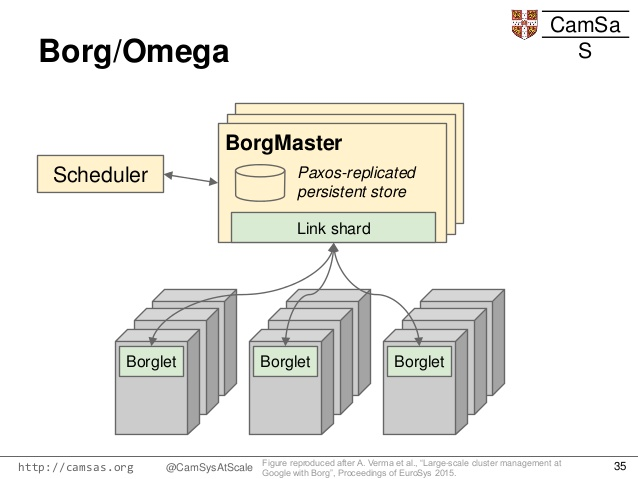
\includegraphics[width=0.9\textwidth]{images/borgArch.jpg}
	\caption{Architektura systemu Borg \cite{borgArchImg}.}
\end{figure}

Powyżej została pokazana architektura omawianego systemu. Każda komórka składa się z wielu połączonych ze sobą maszyn oraz posiada kontroler główny {\it Borgmaster} i zespół agentów {\it Borglet}, które są węzłami na których uruchamiane są kontenery aplikacji. Wszystkie te komponenty zostały napisane w języku C++ w celu optymalizacji i jak najlepszej ich integracji z systemem. Borg zarządza pulą maszyn, a także tym, jakie systemy na nich pracują, ile zasobów potrzebują, oraz metodologią najbardziej efektywnego upakowania maszyn. Jak wspominają przedstawiciele Google, jeśli mamy mniej ważne i bardziej ważne zadania na tej samej maszynie, to możemy zarządzać nimi w sposób bardzo dynamiczny, zabierając i oddając ten sam zestaw zasobów z korzyścią dla systemu, który w danej chwili bardziej go potrzebuje. Borg zarządza też cyklem życia maszyn fizycznych. Informuje, gdy trzeba je naprawić. Wówczas znajdujące się na niej procesy automatycznie przenoszone są na inny serwer. \\ \\
Opis poszczególnych komponentów, z których zbudowany jest Borg przedstawiony został poniżej: \\ \\
{\bf Borgmaster:} Główny komponent każdej komórki systemu Borg. Nasłuchuje on i przetwarza wszystkie żądania klientów i na ich podstawie tworzy nowe zadania lub umożliwia odczytanie danych. Zarządza on również stanem maszyn oraz umożliwia komunikację z Borgletami. Mimo iż ten komponent uruchamiany jest jako pojedyczny proces to jest on replikowany pięć razy w obrębie jednej komórki. Każdy proces posiada podpięty logiczny dysk  bazujący na systemie Paxos19 w celu zachowania stanu systemu. Pozwala on na stworzenie systemu wysokiej dostępności, który zachowuje stan komórki w pamięci. Dodatkowo jeden z procesów jest wybierany jako lider, który jako centralny proces zarządza tworzeniem oraz kończeniem wszelkich zadań. Poprzez zastosowanie odpowiednich mechanizmów, nawet w przypadku błędu procesu lidera, system zachowuje działanie i w ciągu 10 sekund od braku kontaktu z liderem wybierany jest nowy lider. \\ \\
{\bf Planista:} Zajmuje się on optymalnym rozlokowaniem tworzonych zadań na dostęp\-nych maszynach. Po zapisaniu każdego zadania jest ono dodawane do kolejki. Następnie zadania są asynchronicznie sprawdzane i przypisywane do maszyn na podstawie algorytmu Round-Robin{\footnote{Round-Robin - algorytm szeregowania dla procesów w systemie operacyjnym.}, poprzez wybieranie zadań według priorytetów i zapewnienie sprawiedliwego rozlokowania zadań. Po wybraniu grupy maszyn, na których możliwe będzie wystartowanie danego zadania, są one poddawane procesowi oceniania. Na podstawie dostępnych zasobów, ilości uruchomionych zadań, a nawet zaplanowanych prac konserwacyjnych liczona jest ocena maszyn i wybierana ta z najlepszym wynikiem. \\ \\
{\bf Borglet:} Lokalny agent uruchomiony na każdej maszynie, której zadaniem jest uruchamianie zadań użytkowników. Zarządza i monitoruje wszystkie procesy na nim uruchomione i odpowiada za ich uruchamianie, zatrzymywanie czy restartowanie w razie potrzeby. Używa odpowiednich opcji jądra systemu w celu zarządzania zasobami oraz informowania głównego komponentu Borgmaster o dostępnych zasobach. Odpowiada na regularne zapytania ze strony Borgmastera, który weryfikuje stan węzła. Jeśli maszyna nie odpowie w wyznaczonym czasie, zostaje oflagowana, a wszystkie zadania na niej uruchomione zostają przeniesione na inne maszyny. W razie przywrócenia łączności wszelkie zduplikowane zadania zostają zatrzymane.

\subsubsection{Architektura Kubernetesa}

W celu konfiguracji Kubernetesa jako zarządcy kontenerów należy na maszynach zainstalować kilka serwisów/komponentów.

\begin{figure}[h]
	\centering
	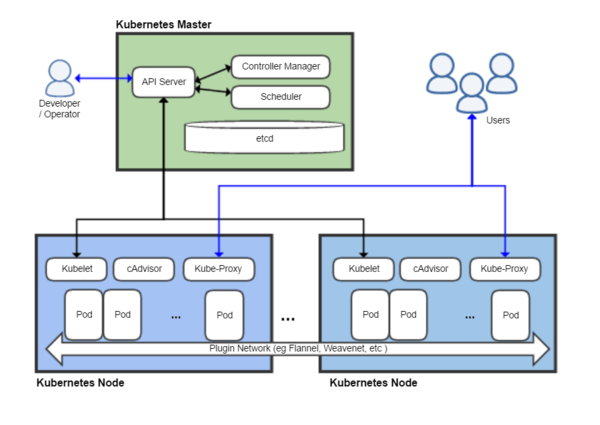
\includegraphics[width=1\textwidth]{images/kubernetesArch.png}
	\caption{Architektura Kubernetesa \cite{kubernetesArchImg}.}
\end{figure}

Jak widać na obrazku przedstawiającym architekturę systemu, komponenty są grupowane pod względem głównego węzła, na którym uruchomiony jest API serwer, kontroler główny, planista oraz istnieje możliwość uruchomienia procesu agenta w celu zarejestrowania węzła głównego również jako maszyny na której można uruchamiać aplikacje. Na pozostałych maszynach uruchomione zostają kolejno agent maszyny, czyli kubelet oraz proces proxy do zapewnienia odpowiedniej łączności z innymi maszynami. Dzięki takiemu podziałowi jesteśmy w stanie jeszcze lepiej utylizować dostępne zasoby i zarządzać klastrem. \\
\\
{\bf Węzeł główny(master)} --- ma za zadanie kontrolować klaster Kubernetesa. Jest to główny węzeł klastra, z którym komunikują się inne węzły jak i użytkownicy. Tylko on powinien być bezpośrednio udostępniony i widoczny dla użytkowników. Ma za zadanie uruchamianie, zarządzanie oraz monitorowanie aplikacji na wszystkich węzłach klastra(nodach), a osiąga to dzięki komunikacji z dodatkowymi komponentami opisanymi poniżej. W szczególności master również może być nodem, czyli węzłem na którym mogą być uruchamiane aplikacje użytkownika.

\begin{itemize}
\item{{\it API serwer} --- jest to kluczowy komponent całego klastra. Jako pośrednik między innymi komponentami, umożliwia użytkownikom konfigurację wszystkich ustawień klastra, od autentykacji, poprzez tworzenie aplikacji, aż po zarządzanie regułami sieciowymi. Pozwala na dostęp do aplikacji uruchomionych na innych węzłach klastra dzięki regułom sieciowym tworzonym przez inny komponent zwany {\it kube-proxy}.}

\item{{\it Kontroler główny} --- jest to demon uruchomiony na masterze w celu obsługi zadań zleconych przez API serwer. Główna pętla aplikacji obserwuje zmiany zachodzące w klastrze. Kiedy taka zmiana następuje, kontroler odczytuje nowy stan obiektu i aktualizuje istniejący obiekt do nowego stanu.}

\item{{\it Planista} --- zarządza on wszystkimi zadaniami i aplikacjami w trakcie ich tworzenia poprzez podejmowanie decyzji, na którym węźle klastra powinny zostać uruchomione. Odpowiednie algorytmy oceniania biorą pod uwagę wiele czynników, takich jak: aktualne obciążenie klastra, dostępne zasoby, planowane prace konserwacyjne i wiele więcej. W razie gdy jeden z węzłów przestanie odpowiadać jego zadaniem jest relokacja aplikacji na nowy węzeł w celu zapewnienia dostępności aplikacji.}

\item{{\it Etcd}: jest to niezawodny i szybki magazyn do przechowywania danych w postaci klucz - wartość. Został stworzony przez firmę CoreOS. Jego głównymi zaletami są: proste API, bezpieczeństwo, szybkość oraz niezawodność. Został napisany w języku Go w oparciu o algorytm Raft \footnote{Raft - algorytm dystrybucji i synchronizacji stanu systemu w klastrze \cite{raft}.}}
\end{itemize}
{\bf Węzeł klastra(node)} --- każdy węzeł klastra wymaga kilku komponentów, które są niezbędne do zapewnienia komunikacji z węzłem głównym i uruchamiania aplikacji. W celu zapewnienia odpowiedniej komunikacji między aplikacjami na różnych węzłach, każdemu z nich przydzielana jest odpowiednia dedykowana podsieć. Poszczególne komponenty zostały opisane poniżej.

\begin{itemize}
\item{{\it Docker} --- pierwszym i najważniejszym wymogiem jest uruchomiony serwis Dockera na każdym węźle klastra, który ma uruchamiać aplikacje. Jest on używany w celu tworzenia aplikacji opartych o kontenery.}

\item{{\it Kubelet} --- ten komponent jest używany w celu zarządzania aplikacjami uruchomionymi na danym węźle. W szczególności zarządza on abstrakcyjnymi obiektami stworzonymi przez Kubernetesa zwanymi podami w celu uproszczenia procesu konfiguracji aplikacji. Funkcjonuje on jako agent, który umożliwia poprzez komunikację z API serwerem na zapisywanie stanu obiektów w magazynie danych etcd. Może on działać niezależnie od głównego węzła, w razie utracenia połączenia, a po jego przywróceniu zaktualizować stan aplikacji w oparciu o informacje uzyskane z mastera. Po pierwszym uruchomieniu rejestruje on węzeł w klastrze, a następnie raportuje zużycie zasobów do mastera, dzięki czemu planista może odpowiednio ocenić dany węzeł w trakcie procesu oceniania.}

\item{{\it Proxy} --- ten komponent uruchomiony jest na każdym węźle klastra i umożliwia ich udostępnienie światu. Jest on odpowiedzialny za tworzenie reguł w tablicy routingu i przekierowywanie żądań do odpowiednich kontenerów aplikacji.}
\end{itemize}
{\bf Dedykowane obiekty Kubernetesa}: Kubernetes tworzy kontenery aplikacji w oparciu o stworzone przez siebie abstrakcyjne obiekty, które mają za zadanie oddzielić zarządzanie aplikacją, tj.: konfigurację sieci w celu udostępnienia aplikacji światu, skalowanie aplikacji czy restartowanie w razie wystąpienia błędów. Poniżej zostały opisane najczęściej używane obiekty. Warto zaznaczyć, że jest ich dużo więcej.

\begin{itemize}
\item{{\it Pod} --- jest podstawowym obiektem tworzonym przez Kubernetesa, który zarządza kontenerami aplikacji. Umożliwia on użytkownikom grupowanie powiązanych ze sobą kontenerów w jeden obiekt. Zamiast uruchamiać wiele zależnych kontenerów i każdą z nich przydzielać do osobnego Poda możemy je uruchomić w obrębie jednego, a Kubernetes będzie nim zarządzać jak jedną aplikacją. Pozwala to na uruchamianie wszystkich zależnych aplikacji w obrębie tego samego węzła klastra, a co za tym idzie współdzielenie zmiennych środowiskowych czy zamontowanych dysków. Dodatkowo kontenery w obrębie jednego Poda posiadają wspólny adres IP. Zazwyczaj Pod zawiera kontener główny, który odpowiada za udostępnianie tzw. frontendu\footnote{Frontend - odpowiedzialny jest za pobieranie danych od użytkownika i przekazywanie ich do backendu, którym zazwyczaj jest serwer, jak również wyświetlanie użytkownikowi danych otrzymanych z backendu. Jest to tzw. warstwa prezentacji danych.} użytkownikowi oraz kontener będący backendem\footnote{Backend - warstwa dostępu do danych. Zazwyczaj jest to serwer, z którym komunikuje się frontend w celu wyświetlenia lub manipulacji danymi.} dla aplikacji głównej.}

\item{{\it Replication controller} --- jest on przede wszystkim zarządcą grupy powiąza\-nych Podów. Jego rolą jest zapewnienie aby zdefiniowana liczba Podów była zawsze uruchomiona w klastrze. Przykładowo, w razie wykrycia zbyt dużej ilości powiązanych Podów usunie nadmiarowe. W odwrotnej sytuacji, jeśli liczba Podów będzie zbyt niska w stosunku do zdefiniowanej, utworzy on nowe. Można go określić jako nadzorcę, który pozwala na łatwe zarządzanie grupą Podów uruchomionych w obrębie klastra.}

\item{{\it Services} --- serwisy są abstrakcyjnymi obiektami, które definiują politykę dostępu do grupy Podów definiujących tą samą aplikację, a posiadających różne adresy IP. Zazwyczaj w celu rozróżnienia, które Pody podlegają pod dany serwis używane są etykiety definiowane przy tworzeniu Podów czy Replication Controllera. W związku z tym, że Pody mogą być usuwane i odtwarzane, co zazwyczaj wiąże się ze zmianą adresu IP, stworzone zostały właśnie serwisy. Dzięki serwisom użytkownik zyskuje dostęp do swojej aplikacji mimo, że może być ona uruchomiona na wielu różnych węzłach klastra. Możemy wyróżnić kilka rodzajów serwisów, które odpowiadają za udostępnianie aplikacji wewnątrz klastra, w obrębie węzła oraz jako Load Balancer\footnote{Load Balancer - technika rozłądowania obciążenia aplikacji poprzez rozproszenie ruchu na wiele procesorów, komputerów czy połączeń sieciowych \cite{cloud}.} w celu udostępnienia aplikacji na świat oraz odpowiedniego kierowania ruchem do naszej aplikacji.}
\end{itemize}

\subsection{Docker Swarm}

Docker Swarm umożliwia tworzenie klastra w oparciu o kontenery Dockera, jednak jego zaletą jest głęboka integracja z samym Dockerem, dzięki czemu jest on natywnie wspierany. Nie jest on tak zaawansowany jak Kubernetes jednak wystarczający do prostych zastosowań. Posiada możliwość grupowania kontenerów w grupy oraz zarządzania nimi w prosty sposób, podobny do zarządzania samymi kontenerami Dockera. Sama architektura jak widać na poniższym obrazku jest dużo prostsza niż w przypadku Kubernetesa. Posiada on planistę oraz Discovery Service, którego zadaniem jest udostępnianie aplikacji oraz umożliwienie komunikacji między aplikacjami wewnątrz klastra, a które uruchomione są na różnych węzłach.

\begin{figure}[h]
	\centering
	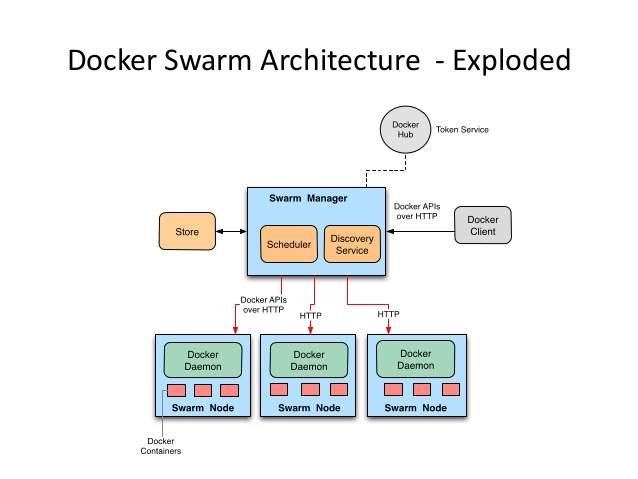
\includegraphics[width=0.9\textwidth]{images/dockerSwarmArch.jpg}
	\caption{Architektura Docker Swarm \cite{dockerSwarmArchImg}.}
\end{figure}

\subsection{Resin.io} \label{subsect:resin}

Resin jest rozwiązaniem przygotowanym w celu przeniesienia zalet kontenerów na mikrokontrolery. Obecnie jako jedyny, umożliwia zdalne uruchamianie kontenerów i zarządzanie grupą mikrokontrolerów ze wspólnego panelu sterowania. Dużą zaletą jest wsparcie wielu różnych urządzeń, od RaspberryPi, aż po Intel NUC. To wszystko pozwala deweloperom skupić się na dostarczeniu samej aplikacji oraz sprzętu, na którym będziemy mogli uruchomić naszą aplikację. Pozostałe kroki wymagane do uruchomienia aplikacji na urządzeniu są zarządzane przez system Resin.io, a są to między innymi:

\begin{itemize}
\item{Przeniesienie kodu na urządzenie.}
\item{Zdalna kompilacja kodu z uwzględnieniem odpowiedniej architektury urządzenia.}
\item{Monitorowanie, zarządzanie i kontrola aplikacji na naszych urządzeniach.}
\item{Zapewnienie bezpieczeństwa komunikacji.}
\item{Dostarczenie środowiska uruchomieniowego dla aplikacji.}
\end{itemize}

Jednak pomimo wielu zalet, nie jest on na tyle zaawansowany i bezpieczny w porównaniu do Kubernetesa. Głównym ograniczeniem jest możliwość uruchomienia jedynie jednego kontenera aplikacji na każdym urządzeniu użytkownika. Grupowanie urządzeń oraz definiowanie zaawansowanych reguł sieciowych w celu ograniczenia komunikacji między urządzeniami również nie jest możliwe \cite{resin}.

\section{Mikrokontroler Raspberry Pi}
Stworzona przez Raspberry Pi Foundation seria mikrokontrolerów Raspberry Pi miała swój początek w Wielkiej Brytanii, gdzie promowane były one jako idealne do nauki podstaw budowy i działania komputerów. Przez lata kolejne modele były ulepszane i obecnie są one używane w zagadnieniach Internetu Rzeczy, robotyce, inteligentnych domach i wielu innych dziedzinach.

\begin{figure}[h]
	\centering
	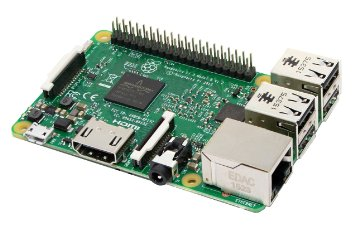
\includegraphics[width=0.81\textwidth]{images/rpi3.jpg}
	\caption{Mikrokontroler Raspberry Pi 3 \cite{rpi3Img}.}
\end{figure}

\clearpage
\noindent Poniższa tabela prezentuje porównanie najpopularniejszych modeli Raspberry Pi, tj.:
\begin{itemize}
\item{Raspberry Pi B+}
\item{Raspberry Pi 2 Model B}
\item{Raspberry Pi Zero}
\item{Raspberry Pi 3 Model B}
\end{itemize}

\noindent W pracy zostały użyte dwa najnowsze obecnie Raspberry Pi 3, w których znaczącej poprawie uległy taktowanie procesora oraz wielkość pamięci RAM. Dzięki temu mogą być one stosowane jako główny węzeł klastra, kontrolujący pozostałe węzły.

\begin{figure}[h]
	\centering
	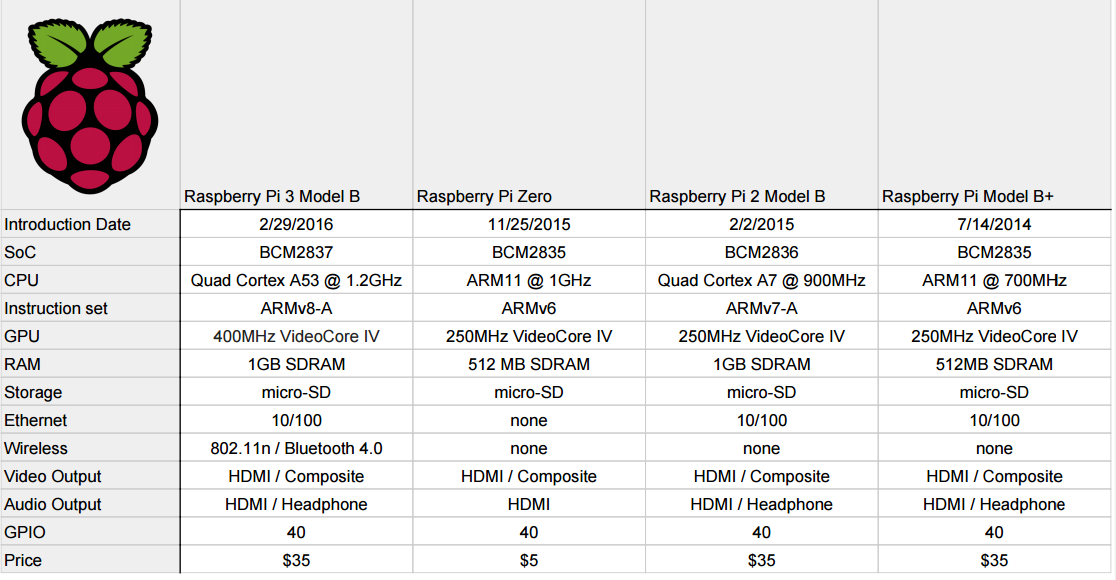
\includegraphics[width=1.05\textwidth]{images/rpiComparison.png}
	\caption{Porównanie najpopularniejszych modeli mikrokontrolera Raspberry Pi \cite{rpiComparisonImg}.}
\end{figure}

\subsection{Protokoły komunikacji}
Poniżej opisane zostały protokoły komunikacji Raspberry Pi, użyte na potrzeby wykonania tej pracy. Protokół SPI użyty został do podłączenia wyświetlacza LED i wyświetlania aktualnej temperatury raportowanej przez czujniki. Jeden z czujników komunikuje się poprzez protokół 1-Wire, natomiast drugi komunikuje się bezpośrednio poprzez piny GPIO. Na rysunku~\ref{fig:pinout} pokazany został układ pinów Raspberry Pi 3.

\begin{figure}[h]
	\centering
	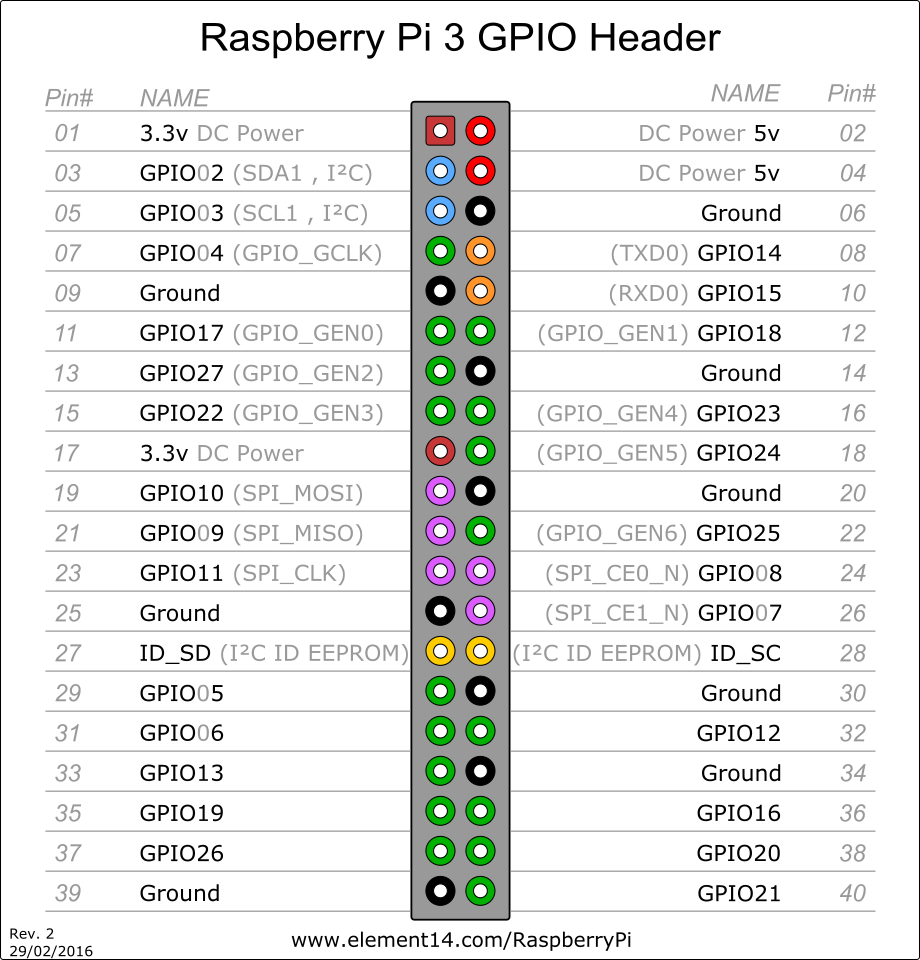
\includegraphics[width=1\textwidth]{images/pi3pinout.png}
	\caption{Układ pinów mikrokontrolera Raspberry Pi 3 \cite{pi3pinoutImg}.}
	\label{fig:pinout}
\end{figure}

\subsubsection{Serial Peripheral Interface - SPI}
Synchroniczny interfejs komunikacji używany głównie przy komunikacji na krótkie dystanse, przeważnie w systemach wbudowanych i mikrokontrolerach. Typowo stosowany do bezpiecznych kart cyfrowych oraz wyświetlaczy LED. \\ \\
Urządzenia komunikujące się przy użyciu interfejsu SPI działają w trybie full duplex, czyli jednoczesnej komunikacji dwukierunkowej. Nadrzędne urządzenie inicjuje komunikację i umożliwia odczyt oraz zapis danych. Dodatkowo możliwa jest komunikacja z wieloma urządzeniami podrzędnymi poprzez wybór odpowiedniej linii sygnałowej \cite{raspberry}.

\subsubsection{1-Wire}
Prosty protokół komunikacyjny, którego nazwa wywodzi się z faktu użycia pojedynczej linii danych do komunikacji. Mimo niskiej prędkości przesyłu danych charakteryzuje się dużą popularnością. Wspiera tzw. zasilanie pasożytnicze, a mianowicie pozwala na zasilanie czujnika bezpośrednio z linii danych. Odbiornik wyposażony w kondensator jest ładowany z linii danych, a następnie ta energia używana jest do zasilania odbiornika. Używany najczęściej w przypadku prostych czujników, np. do raportowania temperatury i wilgotności otoczenia \cite{raspberry}.

\subsubsection{General Purpose Input/Onput - GPIO}
Interfejs ten służy do komunikacji między różnymi elementami systemu, takimi jak mikroprocesor czy urządzenia peryferyjne. Fizycznie komunikacja odbywa się przy użyciu pinów wbudowanych w dane urządzenie, które mogą pełnić rolę wejść i wyjść w zależności od konfiguracji. Często grupowane są one w porty , gdzie jeden port stanowi zazwyczaj osiem pinów GPIO. \\ \\
Komunikacja odbywa się poprzez ustawienie stanu wysokiego lub niskiego na odpowiednim pinie GPIO. Z tego względu pojedynczy pin może służyć jedynie do prostych czynności takich jak wykrywanie zdarzeń, gazów. Natomiast sterowanie grupą pinów jako portem daje dużo większe możliwości \cite{raspberry}.
\chapter{Projekt KubePi} \label{project}
\section{Analiza wymagań}
W tej części zostanie przedstawiona analiza, konfiguracja oraz implementacja systemu KubePi. W pierwszej części zdefiniowane zostają wymagania aplikacji oraz opisane wymagania funkcjonalne wraz z ograniczeniami projektu. Kolejna część opisuje technologie użyte przy tworzeniu projektu. Następnie przedstawiona zostaje propozycja i architektura systemu wraz z opisem implementacji przykładowych aplikacji. Przybliżone zostają kluczowe elementy konfiguracji systemu wraz z opisem kodu najważniejszych elementów aplikacji.

\subsection{Studium możliwości}
Główną ideą projektu jest rozwiązanie problemu stworzenia rozproszonego systemu wysokiej dostępności opartego na architekturze ARM i mikrokontrolerach. Zaletami takiego rozwiązania jest obniżenie kosztów budowy klastra kosztem wydajności. Jednak ze względu na charakter przedsięwzięcia i użycie mikrokontrolerów Raspberry Pi do projektu monitorowania otoczenia, możemy pozwolić sobie na takie ustępstwa, ponieważ wydajność nie jest kluczowa, a stabilność systemu przy odpowiedniej architekturze pozostaje na tym samym poziomie. Dodatkowo po przygotowaniu takiego systemu używanie, zarządzanie i konfiguracja stają się bardzo proste.

\subsection{Wymagania funkcjonalne}
Ze względu na swój charakter oraz wymóg komunikacji między aplikacjami znajdują\-cymi się na różnych węzłach klastra system musi spełniać następujące wymagania:

\begin{enumerate}
\item{Możliwość komunikacji między węzłami klastra.}
\item{Możliwość komunikacji między aplikacjami znajdującymi się na tych samych i różnych węzłach klastra.}
\item{Zarządzanie klastrem i aplikacjami powinno być proste i przejrzyste.}
\item{System powinien zachowywać swój stan w przypadku niezamierzonego restartu systemu.}
\item{W przypadku restartu system powinien samoczynnie wrócić do stanu z przed restartu bez ingerencji użytkownika.}
\end{enumerate}

Dodatkowo system powinien umożliwiać bezpieczny sposób komunikacji z klastrem oraz autentykację i autoryzację użytkowników. Ze względu na obecny poziom skomplikowania pracy ten element zostanie pominięty, jednak system będzie umożliwiał odpowiednią konfigurację zabezpieczeń klastra.
\subsection{Ograniczenia projektu}
Ze względu na skomplikowany proces konfiguracji systemu i klastra, projekt nie będzie umożliwiał łatwego przeniesienia i uruchomienia w innej podsieci. Wymóg stosowania odpowiedniej topologii i narzędzi do zarządzania siecią w celu umożliwienia odpowiedniej komunikacji między elementami systemu wymaga aby urządzenia miały przydzielany stały adres IP lub minimalnie adres z wcześniej skonfigurowanego zakresu podsieci. Ta opcja jednak wymagałaby dodatkowych kroków i odpowiedniej konfiguracji serwera DNS, co nie zostało uwzględnione w tym projekcie.

\section{Sprzęt i technologie}
\subsection{Mikrokontrolery}
Na potrzeby projektu i budowy klastra zostały użyte dwa mikrokontrolery Raspberry Pi 3. Na obu mikrokontrolerach zainstalowany został darmowy system HypriotOS \footnote{HypriotOS - darmowy system przeznaczony na mikrokontrolery Raspberry Pi z wbudowaną obsługą kontenerów Dockera \cite{hypriotos}.}, który natywnie wspiera Dockera i jest dobrze przygotowany do obsługi Kubernetesa. Jeden z mikrokontrolerów został użyty jako główny węzeł klastra, a zarazem jednostka sterująca i zarządzająca klastrem. Druga płytka natomiast została użyta jako dodatkowy węzeł klastra. Ilość węzłów klastra może być bez problemu zwiększona. Kubernetes w najnowszej obecnie wersji, tj. \textit{1.6} może obsłużyć nawet do 5000 węzłów. 
\subsection{Urządzenia peryferyjne}
\subsubsection{DHT11}
Popularny czujnik temperatury i wilgotności powietrza z interfejsem cyfrowym, jednoprzewodowym. Zakres pomiarowy: temperatura 0 \textdegree{}C - 50 \textdegree{}C , wilgotność 20 - 90 \%RH \cite{dht11Botland}. % BOTLAND
\begin{figure}[h]
	\centering
	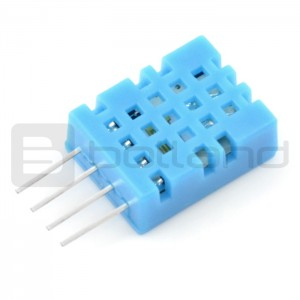
\includegraphics[width=0.3\textwidth]{images/dht11.jpg}
	\caption{Czujnik temperatury i wilgotności DHT11 \cite{dht11Img}.}
\end{figure}
\subsubsection{DS18B20}
Cyfrowy czujnik temperatury DS18B20 z interfejsem 1-wire. Działa w zakresie od -55 \textdegree{}C do 125 \textdegree{}C. Zasilany jest napięciem od 3,0 V do 5,5 V \cite{ds18b20Botland}. % BOTLAND
\begin{figure}[h]
	\centering
	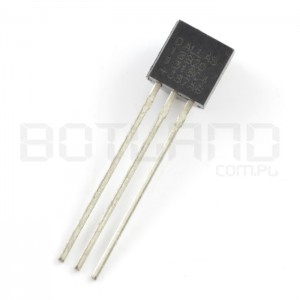
\includegraphics[width=0.3\textwidth]{images/ds18b20.jpg}
	\caption{Czujnik temperatury DS18B20 \cite{ds18b20Img}.}
\end{figure}
\subsubsection{MAX7219}
Moduł matrycy złożonej z 128 czerwonych diod LED ułożonych w prostokąt 16 x 8 pikseli. Płytka posiada zamontowane złącza dopasowane do pinów GPIO Raspberry Pi \cite{max7219Botland}. % BOTLAND
\begin{figure}[h]
	\centering
	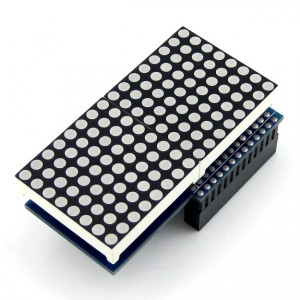
\includegraphics[width=0.3\textwidth]{images/max7219.jpg}
	\caption{Matryca LED MAX7219 (16x8) \cite{max7219Img}.}
\end{figure}
\subsubsection{MQ3}
Czujnik alkoholu z wyjściem analogowym. Mierzy zawartość alkoholu np. w wydychanym powietrzu. \cite{mq3Botland}. % BOTLAND
\begin{figure}[h]
	\centering
	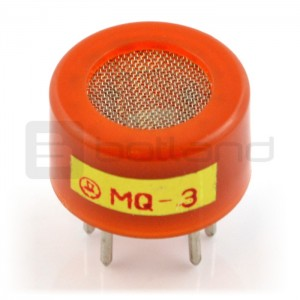
\includegraphics[width=0.3\textwidth]{images/mq3.jpg}
	\caption{Czujnik alkoholu MQ3 \cite{mq3Img}.}
\end{figure}
\subsection{Języki programowania}
Do stworzenia aplikacji przykładowych wybrany został język Go. Najważniejszym czynnikiem decydującym za tym wyborem była obecność dużej ilości bibliotek ułatwiających komunikację ze sprzętem oraz łatwa kompilacja aplikacji przeznaczonych na różne architektury, w tym architekturę ARM. Dodatkowym czynnikiem decydującym o wyborze języka Go jest domyślna kompilacja aplikacji do statycznego pliku binarnego, który nie wymaga dodatkowych zależności, a co za tym idzie w prosty sposób może zostać uruchomiony w kontenerze Dockera. Ostatnią zaletą jest mała zajętość pamięci i czasu procesora w porównaniu z językami takimi jak Java, co jest bardzo ważne przy uruchamianiu aplikacji w kontenerze na mikrokontrolerach typu Raspberry Pi.\\ \\
Dodatkowo w celu stworzenia aplikacji webowej użyta została biblioteka ReactJS. Głównym atutem przemawiającym za wyborem tej biblioteki była popularność, duże wsparcie ze strony społeczeństwa oraz niewielki rozmiar i prostota użycia.

\subsection{Biblioteki}
Do stworzenia aplikacji przykładowych użytych zostało kilka otwartoźródłowych bibliotek dostępnych na portalu Github. Poniżej pokrótce została opisana każda z nich:
\begin{itemize}
\item{\textit{go-restful} --- Jedna z najpopularniejszych bibliotek dla języka Go używanych do tworzenia tak zwanych RESTful Webservices\footnote{RESTful Webservice - rodzaj serwera aplikacji korzystający z architektury REST i udostępniający API zgodne ze standardem REST.} \cite{gorestful}.}
\item{\textit{go-rpio} --- Mała biblioteka pozwalająca w prosty sposób na obsługę pinów GPIO mikrokontrolerów Raspberry Pi. Użyta przy tworzeniu aplikacji do wykrywania alkoholu \cite{gorpio}.}
\item{\textit{go-dht} --- Biblioteka wspierająca czujniki temperatury i wilgotności DHT11 i DHT22. Pozwala na odczyt pomiarów czujnika na mikrokontrolerach Raspberry Pi \cite{godht}.}
\item{\textit{goDS18B20} --- Podobnie do biblioteki \textit{go-dht} pozwala na odczyt pomiarów czujnika temperatury \textit{DS18B20} \cite{gods18b20}.}
\item{\textit{spidev} --- Biblioteka pozwalająca na obsługę urządzeń wykorzystujących interfejs komunikacyjny SPI. Użyta do obsługi wyświetlacza led \textit{MAX7219} \cite{spidev}.}
\item{\textit{ReactJS} --- Biblioteka stworzona przez firmę Facebook napisana w języku JavaScript, pozwalająca w prosty sposób tworzyć interfejs graficzny aplikacji internetowych \cite{reactJSDoc}.}
\end{itemize}
\subsection{Inne narzędzia}
\subsubsection{Flannel}
Jest menadżerem wirtualnej sieci, który umożliwia stworzenie wirtualnej podsieci dla każdego węzła w klastrze. W dużym uproszczeniu pozwala on na komunikację między aplikacjami znajdującymi się w kontenerach uruchomionych na różnych węzłach klastra, przy czym nie jest wymagane aby węzły klastra przebywały w tej samej podsieci. Dzięki takim narzędziom jak Flannel, zwanym \textit{Overlay Networks} możliwa jest komunikacja między aplikacjami uruchomionymi w rozproszonym klastrze \cite{flannel}.
\subsubsection{Kubernetes Dashboard}
Jest to otwartoźródłowy projekt zapoczątkowany przez firmę Google, który ma na celu umożliwienie zarządzania klastrem Kubernetesa z poziomu przeglądarki. Pozwala użytkownikom na zarządzanie aplikacjami uruchomionymi w klastrze, monitorowanie ich stanu, przeglądanie logów oraz uruchamianie nowych aplikacji.
\subsubsection{Github}
Dodatkowym narzędziem użytym w procesie tworzenia aplikacji był system kontroli wersji o nazwie GIT. Pozwalało to kontrolować cały proces powstawania KubePi. Całość jest zintegrowana z portalem Github i przechowywana na prywatnym repozytorium \cite{kubepi}.
\begin{figure}[h]
	\centering
	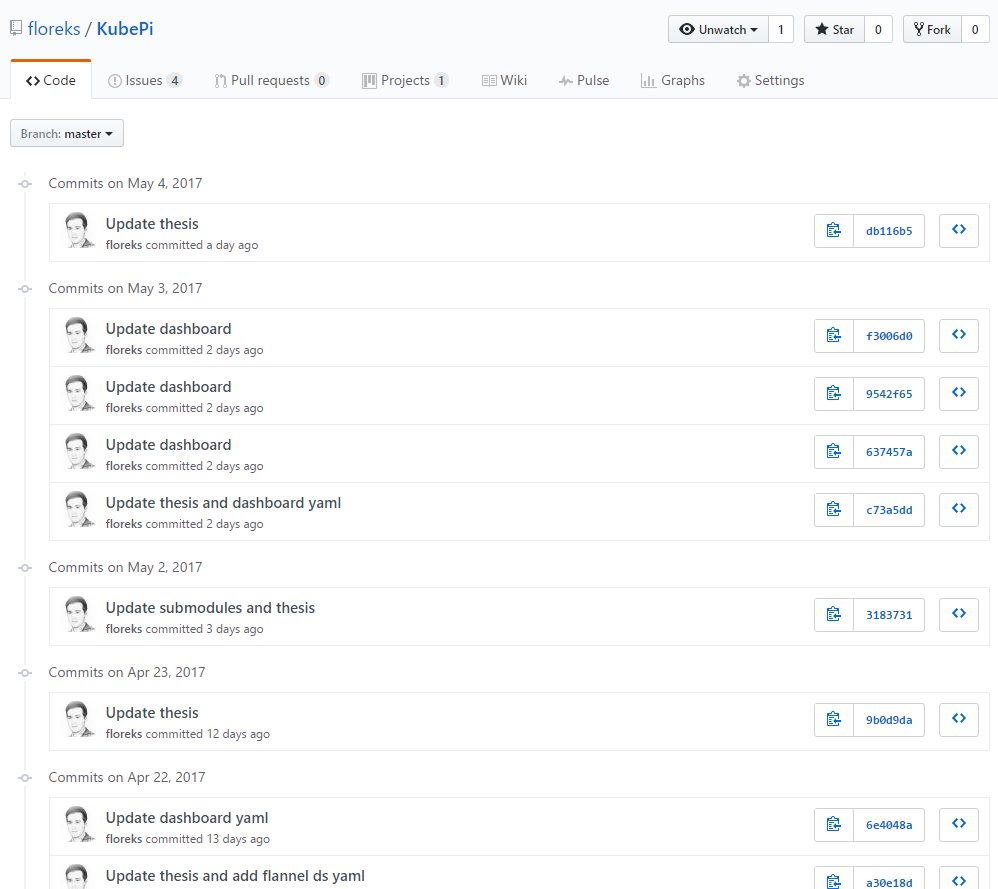
\includegraphics[width=1\textwidth]{images/github.png}
	\caption{Log kontrolny zmian projektowych z portalu Github.}
\end{figure}
\FloatBarrier
\clearpage

\section{Projekt}
\subsection{Architektura systemu}
W tej sekcji przedstawiona zostanie architektura tworzonego systemu oraz schemat połączeń sensorów z płytkami Raspberry Pi. Na poniższym rysunku zobaczyć możemy ogólną architekturę systemu wraz rozkładem uruchomionych procesów. \\
Na głównym węźle klastra uruchomione są wszystkie procesy zarządzające klastrem czyli:
\begin{itemize}
\item{api-server}
\item{kube-scheduler}
\item{kube-controller-manager}
\item{kube-proxy}
\item{kubelet}
\end{itemize}

Dodatkowo uruchomiony jest proces demon \textit{flanneld}, którego zadaniem jest utworzenie wirtualnej podsieci dla klastra. Możemy również zauważyć podłączone sensory z uwzględnieniem konkretnych interfejsów przy użyciu których komunikują się one z urządzeniem.


\begin{figure}[h]
	\centering
	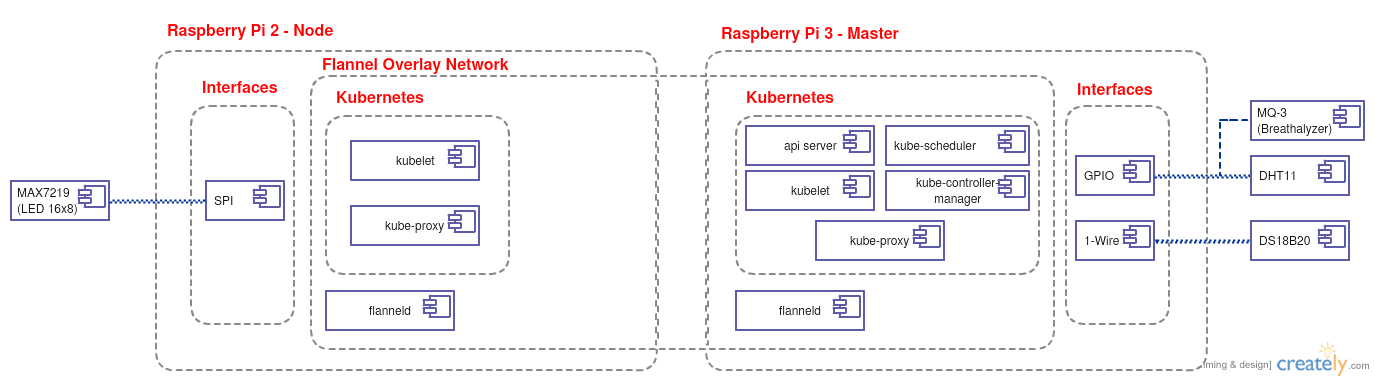
\includegraphics[height=0.41\textwidth, angle=90]{images/KubePi-Architecture.png}
	\caption{Architektura systemu KubePi.}
\end{figure}
\FloatBarrier	

Poniższy schemat obrazuje szczegółowo w jaki sposób konkretne sensory zostały podłączone do mikrokontrolera Raspberry Pi 3. W prawym górnym rogu znajduje się czujnik gazów MQ-3 służący jako wykrywacz alkoholu. Niebieski sensor znajdujący się po lewej stronie to czujnik temperatury i wilgotności DHT11, natomiast najmniejszy sensor znajdujący się na środku to czujnik temperatury DS18B20.

\begin{figure}[h]
	\centering
	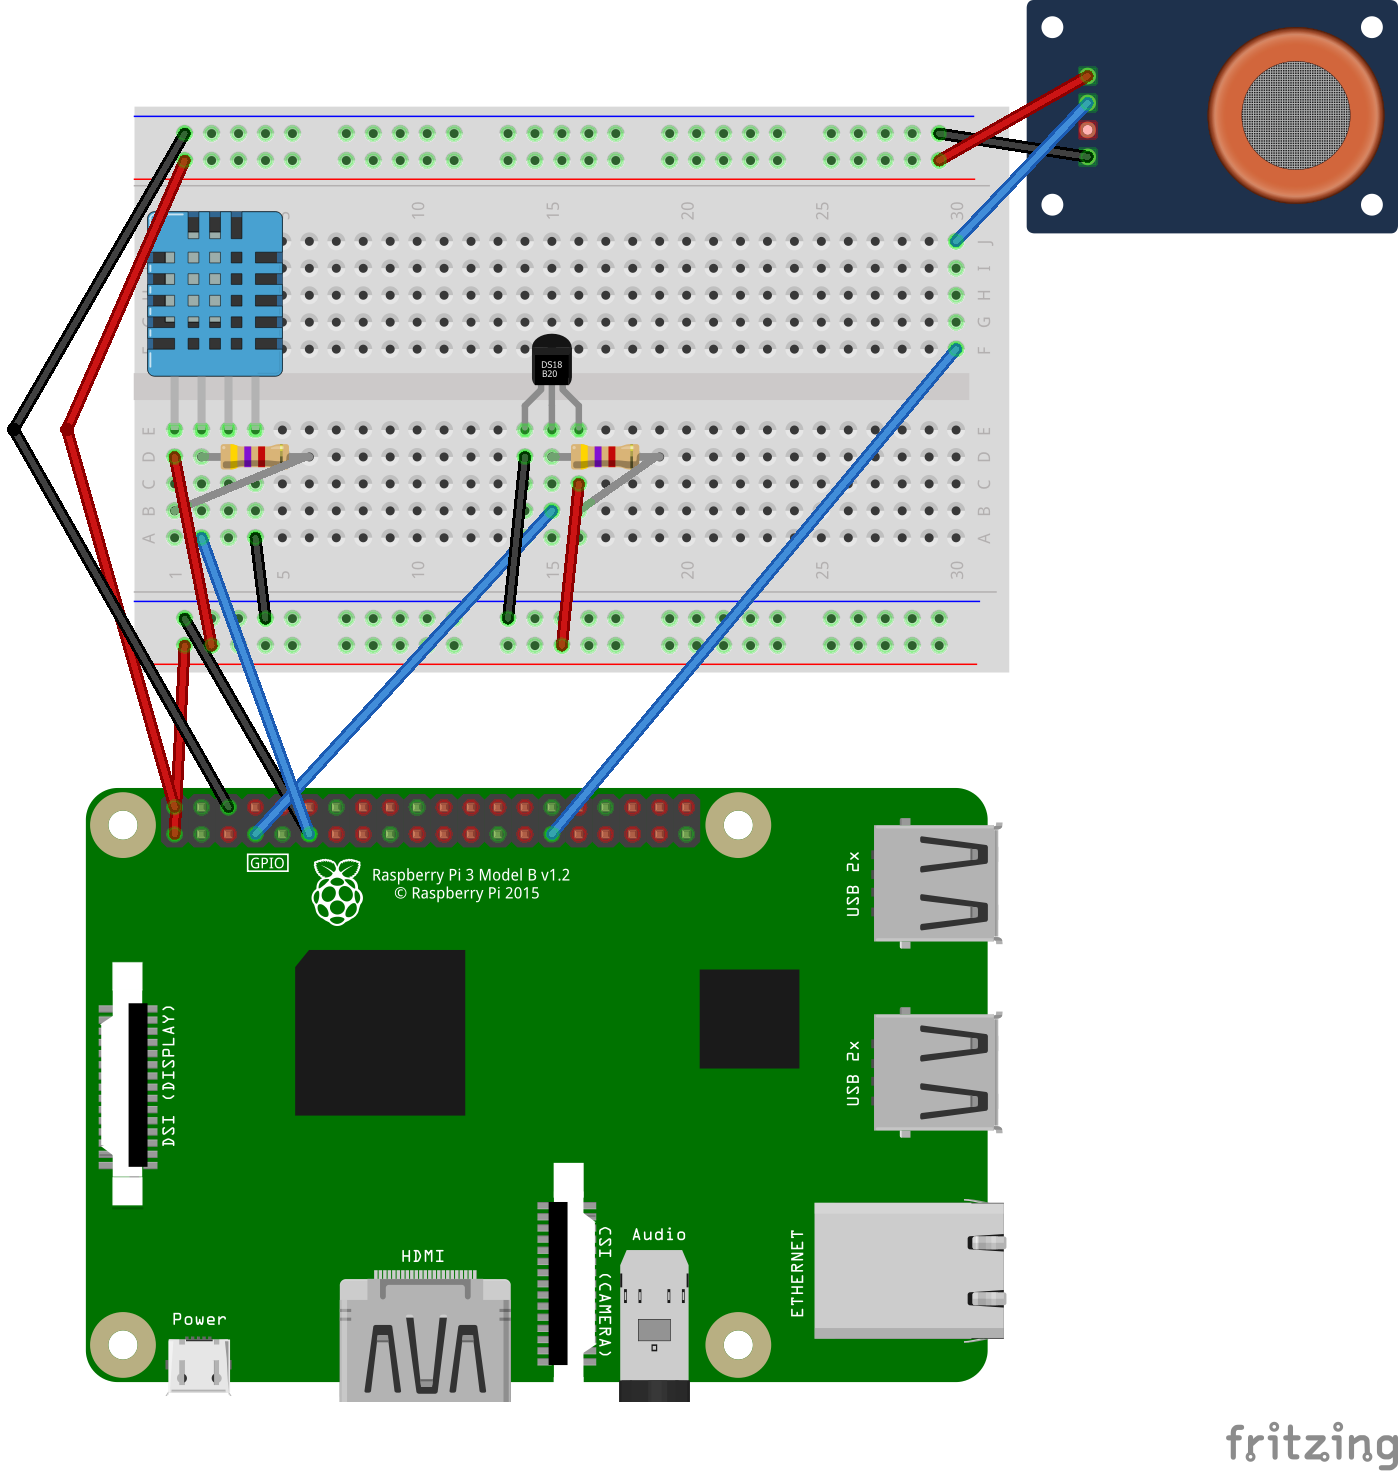
\includegraphics[width=0.99\textwidth]{images/rpi-master.png}
	\caption{Schemat podłączenia sensorów do płytki Raspberry Pi 3.}
\end{figure}
\FloatBarrier	

Ostatnie zdjęcie pokazuje podłączenie matrycy LED mającej za zadanie wyświetlać aktualną temperaturę. Ze względu na dużą ilość kabli zrobione zostało jedynie zdjęcie poglądowe. Użyty moduł można również wpiąć bezpośrednio w płytkę Raspberry Pi bez użycia dodatkowych kabli, co zostało pokazane w końcowym etapie pracy po uruchomieniu całego systemu i wszystkich aplikacji na rysunku~\ref{fig:led}. 

\begin{figure}[h]
	\centering
	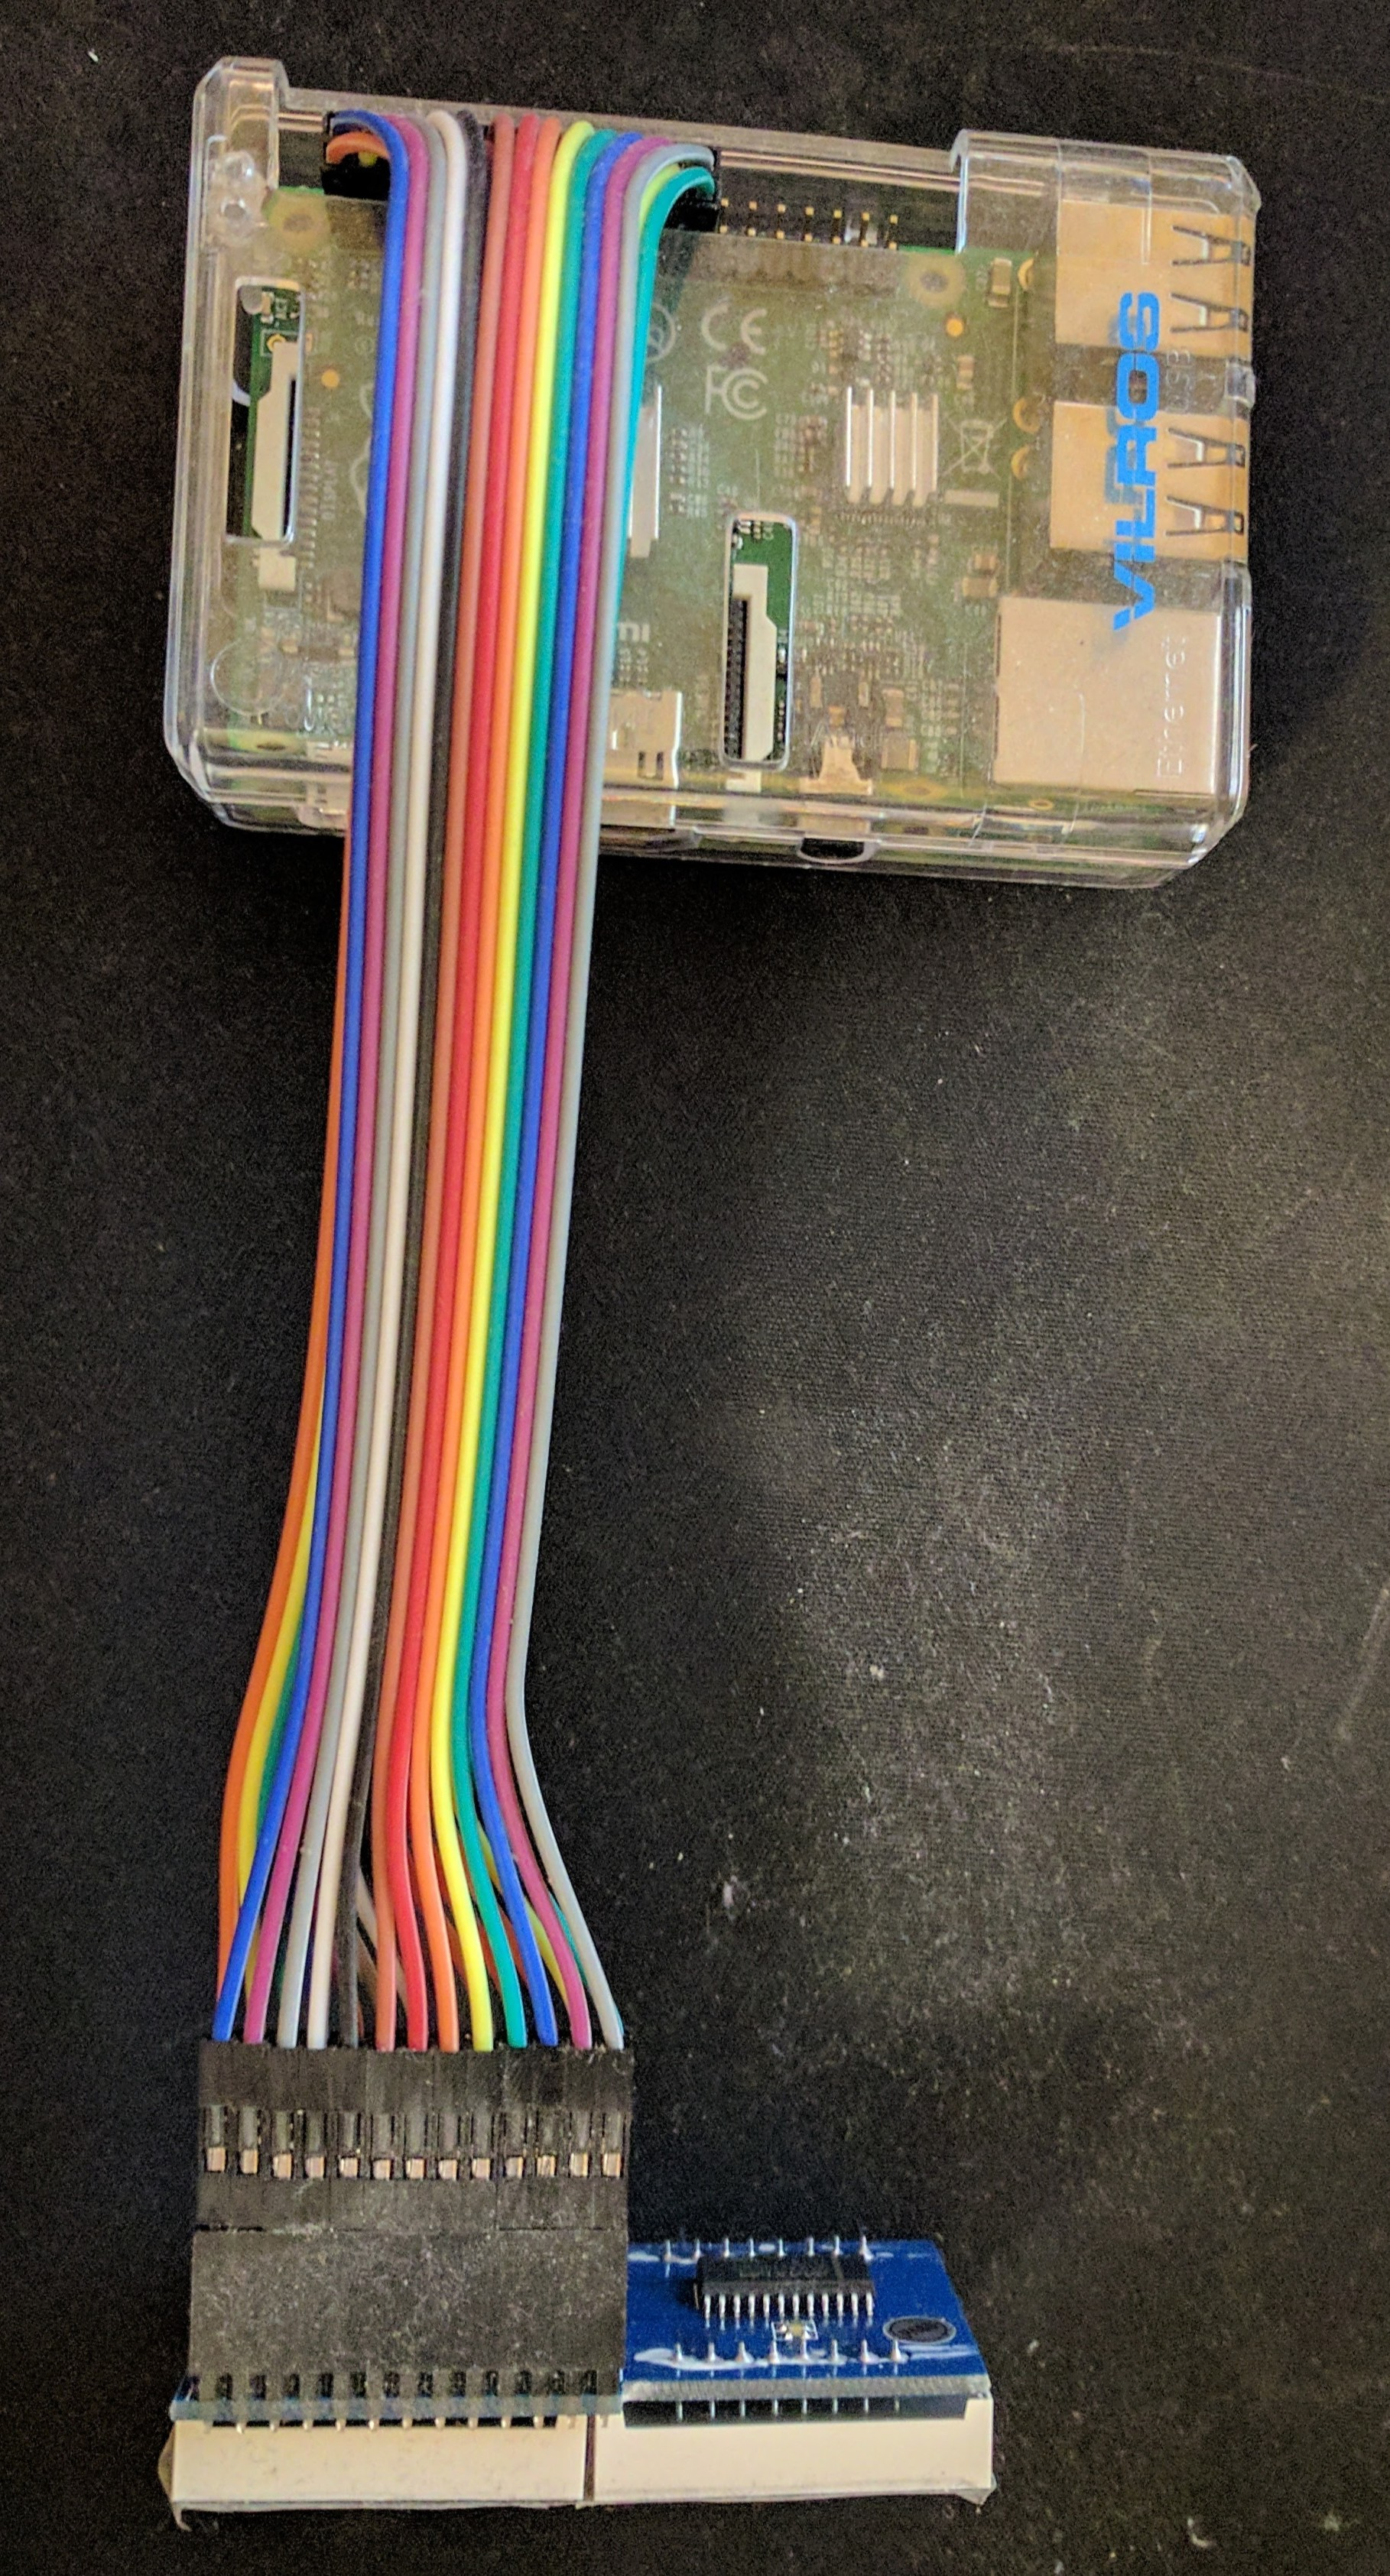
\includegraphics[height=1\textwidth]{images/rpi-node.jpg}
	\caption{Zdjęcie podłączenia matrycy LED 16x8 MAX7219 do płytki Raspberry Pi 3.}
\end{figure}
\FloatBarrier	
\subsection{Przygotowanie i konfiguracja Raspberry Pi}
\subsubsection{Instalacja systemu}
Pierwszym krokiem będzie zainstalowanie systemu HypriotOS \cite{hypriot}. W tym celu należy ściągnąć i wypakować obraz systemu z oficjalnej strony. Dla potrzeb pracy użyty został system w wersji \textit{1.1.3} jednak nowsze obrazy również powinny działać. W wersji 1.1.3 występuje problem z interfejsem \textit{1-Wire}, który trzeba ręcznie naprawić po instalacji. Możliwe, że w nowszych wersjach problem ten jest również obecny.

Następnym krokiem będzie instalacja obrazu na karcie SD. Bardzo dobrym programem dostępnym na większość systemów jest Etcher \cite{etcher}.

Przed pierwszym uruchomieniem możemy zmodyfikować nazwę hosta systemu oraz opcjonalnie ustawić domyślne połączenie z siecią WiFi. W tym celu należy wyszukać na urządzeniu plik o nazwie \textit{device-init.yaml}, a następnie zmienić \textit{hostname} oraz jeśli chcemy aby urządzenie używało sieci WiFi odkomentować i zmienić domyślne ustawienia. Poniżej możemy zobaczyć przykładową zawartość pliku \textit{device-init.yaml}.

\begin{lstlisting}[language=yaml]
# hostname for your HypriotOS device
hostname: kube-master

# optional wireless network settings
wifi:
  interfaces:
     wlan0:
       ssid: "test"
       password: "test"
\end{lstlisting}

\subsubsection{Pierwsze uruchomienie}
W celu wykonania następnych operacji musimy mieć dostęp do systemu zainstalowanego na urządzeniu. Jedną z możliwości jest podłączenie myszy, klawiatury oraz wyświetlacza HDMI do naszego urządzenia jednak nie jest to zbyt wygodne rozwiązanie. Drugą opcją jest znalezienie adresu IP jaki został przydzielony urzą\-dzeniu i komunikacja przy użyciu protokołu SSH. Na systemach linux do znalezienia IP możemy użyć polecenia \textit{nmap}. Więcej informacji o jego użyciu można znaleźć na stronie systemu HypriotOS. Najprostszym sposobem jednak jest zalogowanie się na stronę naszego domowego routera i sprawdzenie listy podłączonych klientów. Nasze urządzenie powinno identyfikować się ustawioną wcześniej nazwą hosta. W moim przypadku jest to nazwa \textit{kube-master}, a urządzeniu przydzielony został adres IP \textit{192.168.0.100}.

\begin{figure}[h]
	\centering
	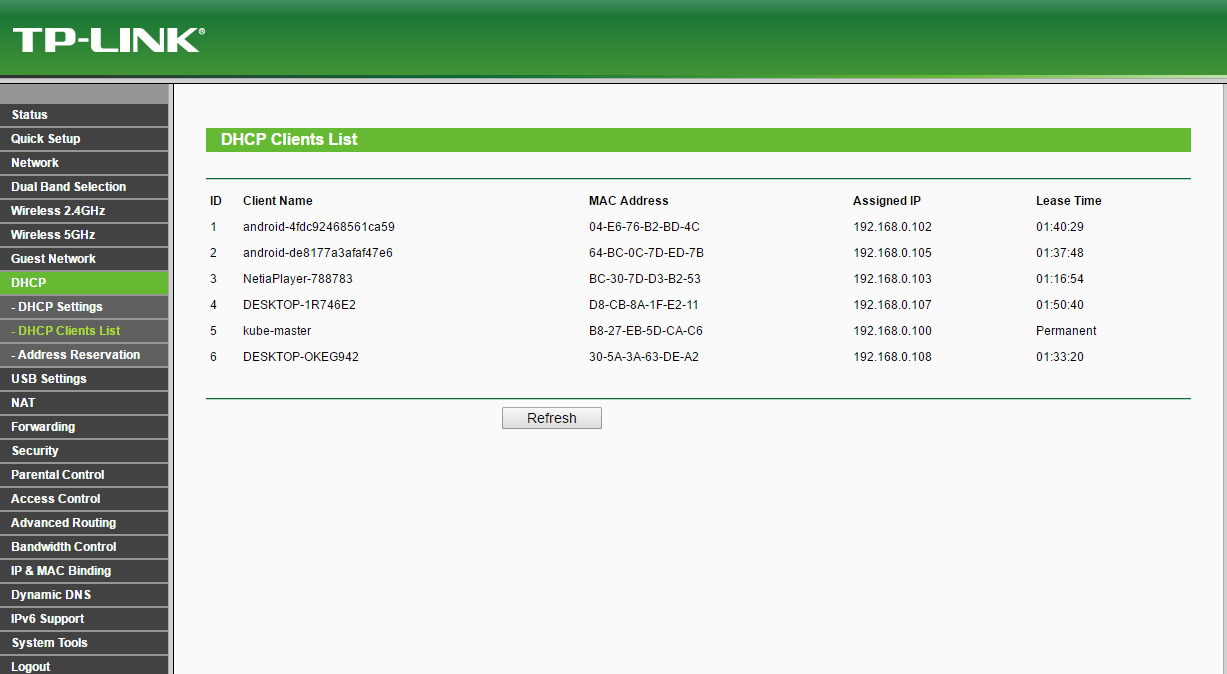
\includegraphics[width=1\textwidth]{images/tp-link-console.png}
	\caption{Konsola admina routera TP-Link.}
\end{figure}
\FloatBarrier

Do połączenia z urządzeniem wykorzystam darmowy program putty\footnote{Putty - aplikacja pozwalająca na połączenie z innymi systemami m.in. przy pomocy protokołu SSH. Strona domowa projektu: \textit{http://www.putty.org/}} służący właśnie do komunikacji z innymi systemami używając między innymi protokołu SSH. Domyśle dane logowania to \textit{pirate:hypriot}. Poniżej możemy zobaczyć zrzut ekranu z programu putty.

\begin{figure}[h]
	\centering
	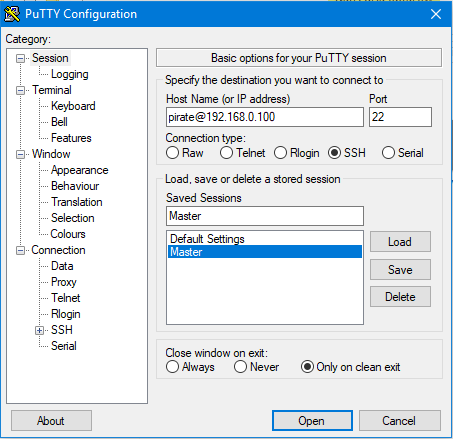
\includegraphics[width=0.9\textwidth]{images/putty.png}
	\caption{Zrzut ekranu z programu putty.}
\end{figure}
\FloatBarrier

\subsubsection{Konfiguracja systemu}
Najpierw należy uruchomić interfejs \textit{1-wire}. W tym celu należy edytować plik \textit{/boot/config.txt} i dodać do niego:

\begin{lstlisting}
dtoverlay=w1-gpio
\end{lstlisting}

Dodatkowo na urządzeniu wykorzystującym matrycę LED Max 7219 należy włączyć interfejs \textit{spi}. Podobnie jak wyżej należy dodać do pliku \textit{/boot/config.txt} następujący wpis:

\begin{lstlisting}
dtparam=spi=on
\end{lstlisting}

Następnie należy uruchomić ponownie urządzenie. Jeśli w folderze \textit{/sys/bus} nie pojawi się folder \textit{w1} oznacza to, że najprawdopodobniej w tej wersji systemu również występuje błąd z ładowaniem sterownika interfejsu \textit{1-wire}. Aby go naprawić należy wykonać następującą komendę i ponownie uruchomić system.

\begin{lstlisting}
sudo mv /boot/overlays/w1-gpio.dtbo	/boot/overlays/w1-gpio.dtb
\end{lstlisting}

\subsection{Instalacja i konfiguracja Kubernetesa} \label{subsect:kubernetes-install}
W celu zainstalowania Kubernetesa skorzystamy z narzędzia o nazwie \textit{kubeadm}, które zostało stworzone w celu uproszczenia procesu instalacji i konfiguracji klastra. Zacznijmy od dodania repozytoriów oraz instalacji \textit{kubeadm}. Wszystkie komendy należy wykonywać jako \textit{root}. \\

\begin{lstlisting}
$ apt-get update && apt-get install -y apt-transport-https
$ curl -s https://packages.cloud.google.com/apt/doc/apt-key.gpg | apt-key add -
$ cat <<EOF >/etc/apt/sources.list.d/kubernetes.list
deb http://apt.kubernetes.io/ kubernetes-xenial main
EOF
$ apt-get update
$ apt-get install -y kubelet kubeadm kubectl kubernetes-cni
\end{lstlisting}

\noindent Kolejnym krokiem jest inicjalizacja głównego węzła klastra. \\

\begin{lstlisting}
$ kubeadm init --pod-network-cidr 10.244.0.0/16
\end{lstlisting}

Ze względu na pobieranie dość dużej ilości proces ten może potrwać kilkanaście minut. Po zakończeniu uruchamiania należy zapisać sobie polecenie służące do dołączania dodatkowych węzłów do klastra. Poniżej możemy zobaczyć przykładowe polecenie. Token zostaje automatycznie wygenerowany i wygasa po określonym czasie.

\begin{lstlisting}
$ kubeadm join --token aed353.f7eb248b374a6ef8 192.168.0.100:6443
\end{lstlisting}

Następnie ustawiamy narzędzie \textit{kubectl}, aby komunikowało się z naszym klastrem.

\begin{lstlisting}
$ mkdir /home/pirate/.kube
$ sudo cp /etc/kubernetes/admin.conf /home/pirate/.kube/config
$ sudo chown -R pirate /home/pirate/.kube
\end{lstlisting}

Następnie już jako użytkownik \textit{pirate} możemy sprawdzić stan klastra.

\begin{lstlisting}[float,floatplacement=H]
$ kubectl get node
NAME          STATUS     AGE       VERSION
kube-master   NotReady   11m       v1.6.1
\end{lstlisting}

Domyślnie główny węzeł klastra jest zablokowany i niemożliwe jest uruchamianie na nim aplikacji. Należy usunąć tą blokadę następującym poleceniem:

\begin{lstlisting}
$ kubectl taint nodes --all node-role.kubernetes.io/master-
\end{lstlisting}

Kolejnym krokiem jest uruchomienie zarządcy sieci, czyli \textit{flannela} w celu umożliwienia komunikacji między aplikacjami w klastrze. Dzięki wykorzystaniu zalet Kubernetesa i stworzeniu \textit{Daemon Seta} na każdym węźle klastra automatycznie zostanie uruchomiona ta aplikacja.

\begin{lstlisting}
$ kubectl create -f https://raw.githubusercontent.com/coreos/flannel/master/Documentation/kube-flannel-rbac.yml
$ kubectl create -n kube-system -f https://raw.githubusercontent.com/floreks/KubePi/master/config/flannel-ds-arm.yaml
\end{lstlisting}

Ostatnim krokiem będzie uruchomienie Dashboardu w celu ułatwienia zarządzania klastrem oraz oznaczenie węzła odpowiednią etykietą dzięki czemu możliwe będzie uruchamianie aplikacji na wybranych przez nas węzłach. 

\begin{lstlisting}[language=bash]
$ kubectl label nodes kube-master target=master
node "kube-master" labeled
$ kubectl create -f https://raw.githubusercontent.com/floreks/KubePi/master/config/dashboard-arm.yaml

# Czekamy na uruchomienie Dashboardu
$ kubectl -n kube-system get pod
NAME                                         READY     STATUS
etcd-kube-master                             1/1       Running
kube-apiserver-kube-master                   1/1       Running
kube-controller-manager-kube-master          1/1       Running
kube-dns-279829092-1fdp6                     3/3       Running
kube-flannel-ds-2ngnl                        2/2       Running
kube-proxy-2kx8h                             1/1       Running
kube-scheduler-kube-master                   1/1       Running
kubernetes-dashboard-head-2455883860-974t0   1/1       Running

# Sprawdzamy port na ktorym wystawiony zostal Dashboard
$ kubectl -n kube-system get service kubernetes-dashboard-head -o template --template="{{ (index .spec.ports 0).nodePort }}"
31143
\end{lstlisting}

Od teraz możemy zarządzać naszym klastrem z poziomu przeglądarki, w naszym przypadku Dashboard dostępny jest pod adresem \textit{192.168.0.100:31143}.

\begin{figure}[h]
	\centering
	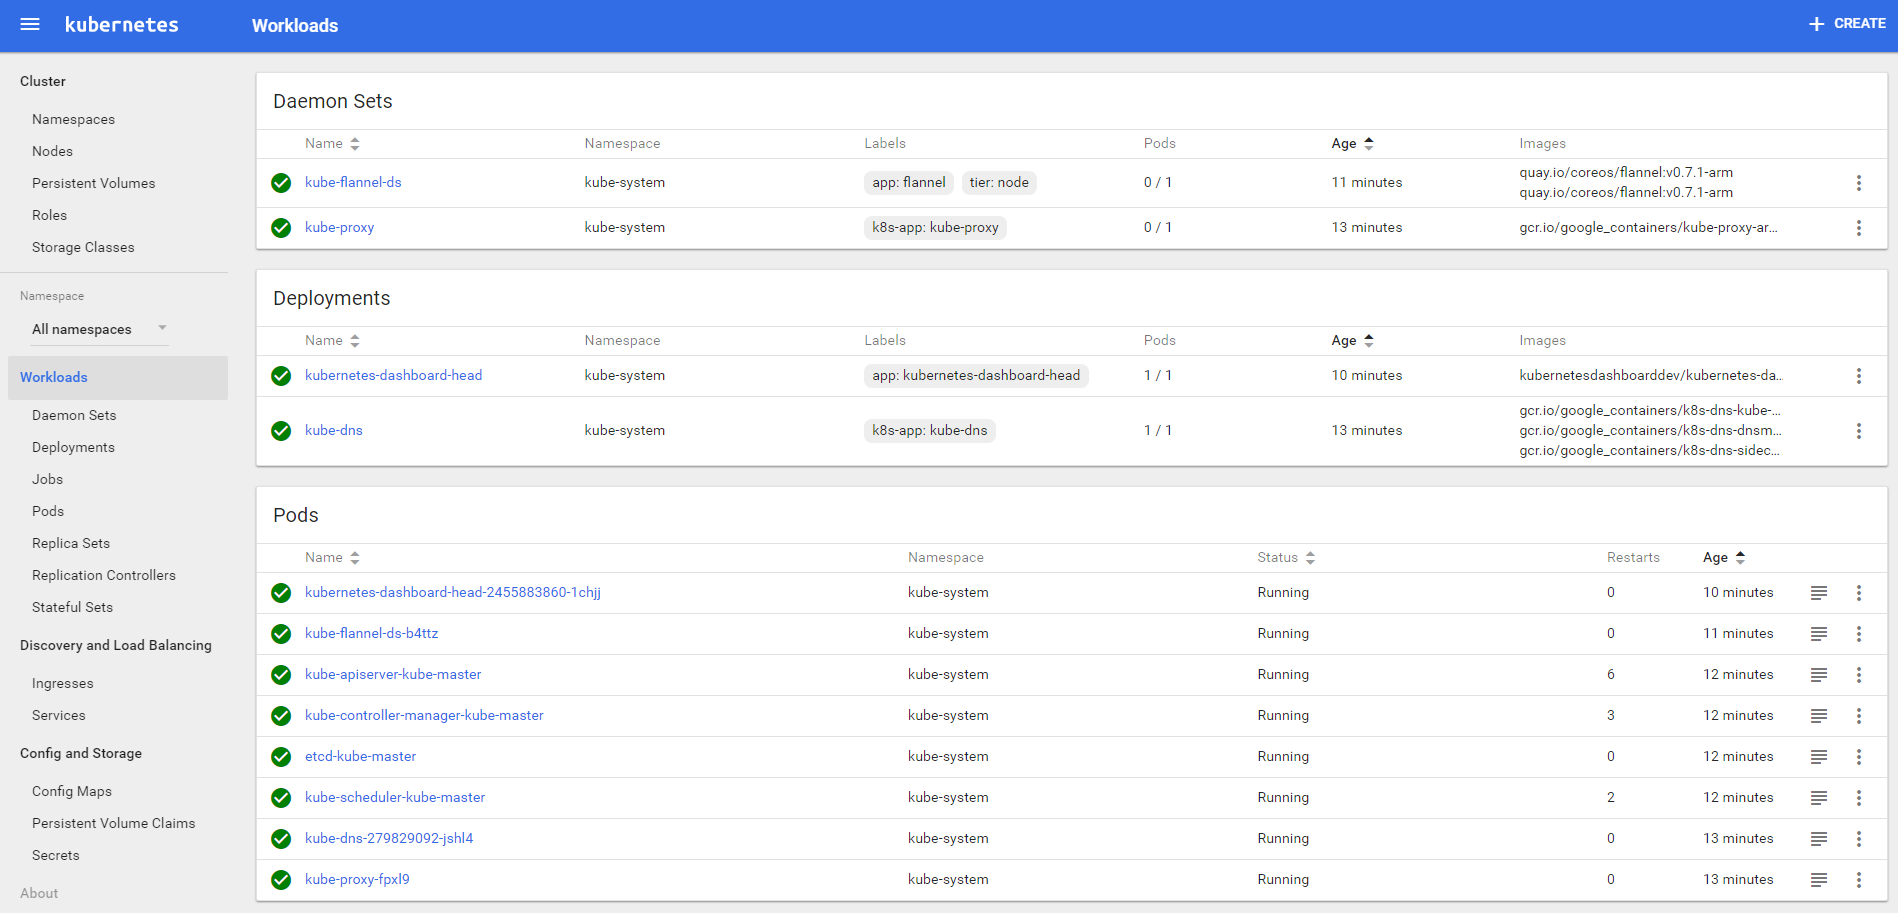
\includegraphics[width=1\textwidth]{images/dashboard.png}
	\caption{Zrzut ekranu z aplikacji Kubernetes Dashboard.}
\end{figure}
\FloatBarrier

Po poprawnym skonfigurowaniu głównego węzła, należy skonfigurować dodatkowy węzeł. W naszym przypadku rolę tą pełnić będzie drugi mikrokontroler Raspberry Pi 3. Ponownie wypalamy obraz systemu HypriotOS, uruchamiamy i podłączamy się używając protokołu SSH. Należy pamiętać o ustawieniu innej nazwy hosta w pliku \textit{device-init.yaml}. Na potrzeby pracy drugi węzeł nazwany został \textit{kube-node}. Na tej maszynie również należy zainstalować narzędzie \textit{kubeadm} w celu podłączenia węzła do klastra. Kiedy wszystko jest gotowe wykonujemy polecenie:

\begin{lstlisting}
$ kubeadm join --token 645058.48480ab896795f04 192.168.0.100:6443
\end{lstlisting}

Po chwili nasz węzeł powinien zostać skonfigurowany i dołączony do klastra. Z poziomu Dashboardu możemy sprawdzić jego status.

\begin{figure}[h]
	\centering
	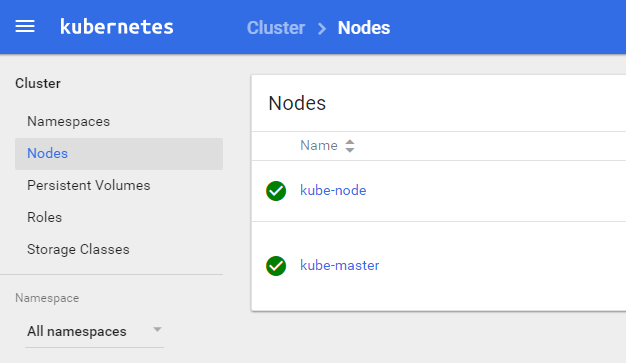
\includegraphics[width=1\textwidth]{images/node_status.png}
	\caption{Zrzut ekranu pokazujący status węzłów klastra.}
\end{figure}
\FloatBarrier

Na koniec oznaczamy nowy węzeł odpowiednią etykietą w celu łatwiejszego zarządzania uruchamianiem aplikacji na konkretnych węzłach.

\begin{lstlisting}
$ kubectl label nodes kube-node target=node-1
node "kube-node" labeled
\end{lstlisting}

\subsection{Projekt aplikacji przykładowych}
W tej sekcji zapoznamy się ze stworzonymi aplikacjami monitorującymi otoczenie. Zwrócimy uwagę na kluczowe elementy implementacji oraz sposób konfiguracji i dystrybucji, który ma na celu uproszczenia procesu uruchamiania aplikacji w klastrze.

\subsubsection{Monitoring Server} \label{subsect:monitoring-server}
Pierwsza aplikacja pełni rolę serwera do monitorowania temperatury i wilgotności. Pozwala na odczyt pomiarów z opisanych wcześniej sensorów DHT11 oraz DS18B20. \\ \\
Listing~\ref{lst:dht-config} przestawia konfigurację całej aplikacji. Dzięki użyciu biblioteki \textit{restful-go} w prosty sposób można stworzyć serwer bazujący na architekturze REST.
\begin{lstlisting}[language=golang,caption=Konfiguracja aplikacji,label=lst:dht-config]
var (
	argPort = pflag.Int("port", 3000, "The port to listen on for incoming HTTP requests")
)

func main() {
	...
	// Parse command line arguments
	pflag.CommandLine.AddGoFlagSet(flag.CommandLine)
	pflag.Parse()

	// Register handler
	restful.Add(dht.NewDHT11Service().Handler())
	restful.Add(ds18b20.NewDS18B20Service().Handler())

	log.Printf("Listening on port: %d", *argPort)
	log.Fatal(http.ListenAndServe(fmt.Sprintf(":%d", *argPort), nil))
\end{lstlisting}

\noindent Listing~\ref{lst:dht-api} przedstawia rejestrowanie odpowiednich podstron, które pozwolą na wykonanie kodu poprzez przejście na odpowiedni adres w przeglądarce. W tym wypadku rejestrujemy podstronę \textit{"/dht11"}, która zwróci nam odczyt z sensora w formacie \textit{JSON}.
\begin{lstlisting}[language=golang,caption=Konfiguracja API,label=lst:dht-api]
func (d DHT11Service) Handler() *restful.WebService {
	ws := new(restful.WebService)
	ws.
		Path("/dht11").
		Consumes(restful.MIME_JSON).
		Produces(restful.MIME_JSON)

	ws.Route(ws.GET("/").To(d.readFromSensor).
		Doc("Reads temperature and humidity from DHT11 sensor").
		Writes(sensor.DHTResponse{}))
\end{lstlisting}

\noindent Na listingu~\ref{lst:dht-apicall} widzimy kod, który zostaje wykonany po przejściu na podstronę \textit{"/dht11"}. Odczyt danych z sensora zostaje oddelegowany do osobnego interfejsu, a w tej części następuje jedynie obsługa błędów i zwrócenie wyniku.
\begin{lstlisting}[language=golang,caption=Wywołanie kodu API,label=lst:dht-apicall]
func (d DHT11Service) readFromSensor(request *restful.Request, response *restful.Response) {
	result, err := d.reader.ReadFromSensor()
	if err != nil {
		service.HandleInternalServerError(response, err)
		return
	}

	response.WriteHeaderAndEntity(http.StatusOK, result)
}
\end{lstlisting}

\noindent Listing~\ref{lst:dht-struct} pokazuje struktury, które zostały zdefiniowane w celu lepszego podziału danych zwracanych przez sensor \textit{DHT11}. \textit{DHTResponse} jest strukturą zwracaną bezpośrednio przez serwer i składa się z temperatury oraz wilgotności. Dodatkowy podział został wprowadzony ze względu na dodanie opcji odczytu pojedynczych wartości temperatury lub wilgotności. Interfejs \textit{DHTReader} natomiast posiada odpowiednie metody do odczytu danych z sensora. Implementacja metod dla sensora \textit{DHT11} znajduję się w osobnym pliku. Dzięki wykorzystaniu interfejsu możliwe jest użycie tych samych struktur do odczytu danych z podobnych sensorów.
\begin{lstlisting}[language=golang,caption=Struktury odpowiedzi serwera,label=lst:dht-struct]
type DHTResponse struct {
	DHTTemperature
	DHTHumidity
}

type DHTTemperature struct {
	// Temperature
	Temperature float32 `json:"temperature"`
}

type DHTHumidity struct {
	// Humidity
	Humidity float32 `json:"humidity"`
}

type DHTReader interface {
	ReadFromSensor() (*DHTResponse, error)
	ReadTemperature() (*DHTTemperature, error)
	ReadHumidity() (*DHTHumidity, error)
	SetGPIO(int)
	ResetGPIO()
}
\end{lstlisting}

\noindent Ostatni listing~\ref{lst:dht-read} przedstawia wykorzystanie biblioteki \textit{go-dht} i bezpośredni odczyt wartości sensora \textit{DHT11} z domyślnie ustawionego 17 pinu GPIO.
\clearpage
\begin{lstlisting}[language=golang,caption=Odczyt danych z sensora DHT11,label=lst:dht-read]
func (DHT11Reader) ReadFromSensor() (*DHTResponse, error) {
	log.Printf("Reading from sensor %s on GPIO pin %d", dht.DHT11, gpioPinOverride)
	temp, humidity, _, err := dht.ReadDHTxxWithRetry(dht.DHT11, gpioPinOverride, BOOST_PERF_FLAG,
		RETRIES)
	if err != nil {
		if strings.Contains(err.Error(), "C.dial_DHTxx_and_read") {
			return nil, fmt.Errorf("Could not read from sensor.")
		}

		return nil, err
	}

	return &DHTResponse{DHTTemperature{Temperature: temp}, DHTHumidity{Humidity: humidity}}, nil
}
\end{lstlisting}

\noindent Aplikacja posiada również opcję nadpisania numeru pinu GPIO, z którego należy odczytać dane. Możliwe jest to dzięki wywołaniu operacji \textit{POST} na podstronie o adresie \textit{"/dht11"} i przesłanie parametru \textit{gpio=x}, gdzie \textit{x} to numer pinu GPIO z którego chcemy odczytywać dane.

\subsubsection{Breathalyzer} \label{subsect:breathalyzer}
Kolejna aplikacja ma za zadanie wykrywanie alkoholu w powietrzu. Po uruchomieniu mierzy przez 5 sekund zawartość alkoholu, następnie uśrednia wynik i informuje użytkownika czy alkohol został wykryty czy nie. Nie posiada ona funkcji dokładnego pomiaru stężenia alkoholu, a jedynie informuje o jego obecności. \\

\noindent Listing~\ref{lst:breathalyzer-api} podobnie do listingu~\ref{lst:dht-api} przedstawia budowanie API naszej aplikacji. Przejście na postronę \textit{"/mq3/measure"} uruchamia pomiar.
\clearpage
\begin{lstlisting}[language=golang,caption=Konfiguracja API,label=lst:breathalyzer-api]
func (d MQ3Service) Handler() *restful.WebService {
	ws := new(restful.WebService)
	ws.
		Path("/mq3").
		Consumes(restful.MIME_JSON).
		Produces(restful.MIME_JSON)

	ws.Route(ws.GET("/measure").To(d.detectAlcohol).
		Doc("Reads temperature from DS18B20 sensor").
		Writes(sensor.MQ3Response{}))

	return ws
}
\end{lstlisting}

\noindent Listing~\ref{lst:breathalyzer-run} pokazuje główną metodę całej aplikacji, której zadaniem jest sprawdzenie obecności alkoholu w powietrzu. Pomiar odbywa się w 5-sekundowym przedziale czasowym z częstotliwością 10 odczytów na sekundę, co pozwala na uzyskanie 50 próbek danych. Dane te są następnie uśredniane, a wykrycie alkoholu sygnalizowane w przypadku jeśli czujnik pozostawał w stanie niskim co najmniej przez połowę okresu próbkowania.
\clearpage
\begin{lstlisting}[language=golang,caption=Pomiar alkoholu w powietrzu,label=lst:breathalyzer-run]
// DetectAlcohol reads for 5 sec digital out from mq-3 sensor and returns true or false based on readings over time
func (this MQ3Reader) DetectAlcohol() MQ3Response {
	timeoutChan := time.NewTimer(this.detectionTimeout).C
	intervalChan := time.NewTicker(this.detectionInterval).C
	var result int
	tmp := 1.0
	readings := this.detectionTimeout.Seconds() / this.detectionInterval.Seconds()
	pin := rpi.Pin(this.gpioPin)
	// Set input mode to read from the pin
	pin.Input()
	for {
		select {
		case <-timeoutChan:
			tmp = tmp / float64(readings)
			result = int(tmp + 0.5)

			if result == 0 {
				return MQ3Response{AlcoholDetected: false}
			}

			return MQ3Response{AlcoholDetected: true}
		case <-intervalChan:
			out := pin.Read()
			if out == rpi.Low {
				tmp += 1.0
			}
		}
	}
}
\end{lstlisting}

\newpage
\subsubsection{Wyświetlacz temperatury}
Zadaniem tej aplikacji jest okresowe pobieranie temperatury poprzez odpytywanie stworzonego wcześniej serwera monitorującego oraz wyświetlanie jej na matrycy LED MAX7219. \\

\noindent Listing~\ref{lst:led-config} przedstawia konfigurację aplikacji. Aplikacja przyjmuje jako parametr adres serwera, z którego pobiera potrzebne dane. W dalszym kroku następuje konfiguracja wyświetlacza oraz startowany jest wątek odpytujący serwer. Komunikacja między wątkami odbywa się poprzez kanały, które są podstawowymi mechanizmami komunikacji między wątkami w języku Go. Po odczytaniu danych z serwera są one zapisywane do kanału \textit{tempChan}, a następnie główny wątek pobiera te dane i wyświetla temperaturę.
\begin{lstlisting}[language=golang,caption=Konfiguracja aplikacji,label=lst:led-config]
func main() {
	dev, err := device.NewMax7219()
	if err != nil {
		...
	}
	err = dev.Init()
	if err != nil {
		...
	}

	defer dev.Close()
	tempChan := make(chan float32)
	
	go pollTemperature(pollServer, tempChan)
	registerSigtermHandler(dev)
	
	for temp := range tempChan {
		err := dev.DisplayTemperature(temp)
		if err != nil {
			...
		}
	}
}
\end{lstlisting}

\newpage
\noindent Następny listing~\ref{lst:led-temp-read} przedstawia proces pobierania temperatury z serwera i zapisywania do struktury \textit{TempResponse}. Co pewien okres czasu, zdefiniowany w zmiennej \textit{POLLING\_TIME} dane pobierane są z serwera. Następnie są one dekodowane do struktury \textit{TempResponse}, która zawiera tylko jedno pole \textit{Temperature}. Po poprawnym zdekodowaniu struktury jest ona przesyłana do kanału \textit{tempChan}, który służy do synchronizacji z głównym wątkiem aplikacji.
\begin{lstlisting}[language=golang,caption=Odczyt temperatury z serwera,label=lst:led-temp-read]
func pollTemperature(pollServer *string, tempChan chan float32) {
	tempResponse := new(TempResponse)

	for {
		r, err := http.Get(*pollServer)
		if err != nil {
			log.Printf("Error durring temperature polling: %s", err.Error())
			os.Exit(1)
		}

		err = json.NewDecoder(r.Body).Decode(tempResponse)
		if err != nil {
			log.Printf("Error during server response decoding: %s", err.Error())
			os.Exit(1)
		}

		tempChan <- tempResponse.Temperature
		time.Sleep(POLLING_TIME)
		r.Body.Close()
	}
}
\end{lstlisting}

\newpage
\noindent Ostatnim i najważniejszym krokiem jest wyświetlenie temperatury, co przedstawia kod w listingu~\ref{lst:led-display}. Temperatura zostaje rzutowana na liczbę całkowitą, ze względu na brak miejsca na wyświetlaczu. Następnie liczba ta konwertowana jest na odpowiednią tablicę bajtów o rozmiarze 2x8. Każdy wiersz reprezentuję cyfrę, która wyświetlana jest na obszarze 8x8. Każda kolumna reprezentuje natomiast pojedynczy wiersz 8 diód na matrycy. Przykładowo wpisanie cyfry 2 (binarnie 00000010) do rejestru 0 spowoduje podświetlenie przedostatniej diody w pierwszym wierszu matrycy LED.
\begin{lstlisting}[language=golang,caption=Wyświetlanie temperatury,label=lst:led-display]
func (this Max7219) DisplayTemperature(temperature float32) error {
	// Round to integer number as we don't have space for floating point numbers
	temp := int(temperature)

	buf, err := DEFAULT_FONT.FromInt(temp)
	if err != nil {
		return err
	}

	for i := 0; i < MAX7219_DIGIT_COUNT; i++ {
		err := this.send(Max7219Reg(i), buf[1][i], buf[0][i])
		if err != nil {
			return err
		}
	}

	return nil
}
\end{lstlisting}

\newpage
\subsubsection{KubePi Monitor} \label{subsect:kubepi-monitor}
Ostatnia aplikacja jest aplikacją webową i pozwala na monitorowanie odczytów sensorów z poziomu przeglądarki. Podobnie do poprzedniej aplikacji pobiera okresowo dane z serwera monitorującego i wyświetla je oraz na żądanie użytkownika startuje wykrywacz alkoholu. \\

\noindent Listing~\ref{lst:kubepi-fetch} przedstawia funkcję służącą do startowania wątku, który okresowo (domyślnie co 3 sekundy) odpytuje serwer przekazany jako parametr funkcji o dane.
\begin{lstlisting}[language=golang,caption=Startowanie wątków do odczytu danych,label=lst:kubepi-fetch]
  runPollInterval(fetchFn, address, timeout = 3000, immediate = true) {
    let intervalId = setInterval(() => {
      this.props.dispatch(fetchFn(address))
    }, timeout, true)

    if(immediate) {
      this.props.dispatch(fetchFn(address))
    }

    return intervalId
  }
\end{lstlisting}

\noindent Funkcja przedstawiona na listingu~\ref{lst:kubepi-dht-read} jest odpowiedzialna za uruchamianie oraz zatrzymywanie wątku pobierającego dane z czujnika temperatury i wilgotności DHT11. Odpytuje ona lokalny serwer o dane, który jest pośrednikiem między częścią webową, a klastrem.
\begin{lstlisting}[language=golang,caption=Startowanie wątku odpytującego nasz serwer o dane z sensora DHT11,label=lst:kubepi-dht-read]
  handleDHT11() {
    if(this.state.dhtIntervalId === 0) {
      let intervalId = this.runPollInterval(dht11.fetchData, '/dht11')
      this.setState({
        dhtIntervalId: intervalId,
      })
    } else {
      clearInterval(this.state.dhtIntervalId)
      this.props.dispatch(dht11.reset())
      this.setState({
        dhtIntervalId: 0,
      })
    }
  }
\end{lstlisting}

\noindent Ostatni listing~\ref{lst:kubepi-dht-go-read} przedstawia funkcję serwera Go, która odpowiedzialna jest za pobieranie odczytów z serwera monitorującego opisanego w sekcji~\ref{subsect:monitoring-server}.
\begin{lstlisting}[language=golang,caption=Odczyt temperatury z naszego serwera,label=lst:kubepi-dht-go-read]
func dht11Handler(w http.ResponseWriter, r *http.Request) {
	dht11Response := new(DHT11Response)

	resp, err := http.Get("http://dht-server.default.svc.cluster.local:3000/dht11")
	if err != nil {
		fmt.Fprintf(w, "Error durring temperature polling: %s", err.Error())
		return
	}

	err = json.NewDecoder(resp.Body).Decode(dht11Response)
	if err != nil {
		fmt.Fprintf(w, "Error during server response decoding: %s", err.Error())
		return
	}

	log.Println(dht11Response)
	w.Header().Set("Content-Type", "application/json")
	json.NewEncoder(w).Encode(dht11Response)
}
\end{lstlisting}
\subsubsection{Budowanie i dystrybucja}
W tej sekcji opisane zostały proces budowania i dystrybucji aplikacji wraz z użytymi narzędziami. \\ \\
Język Go pozwala na łatwe budowanie aplikacji do pojedynczego pliku wykonywalnego. Użycie aplikacji \textit{xgo} \cite{xgo}, pozwoliło uprościć proces budowania aplikacji na różne architektury. Budowanie aplikacji na inne architektury odbywa się w kontenerze Dockera, który został wcześniej skonfigurowany i zawiera wszystkie zależności potrzebne do budowania aplikacji. Domyślnie korzysta on z kompilatora języka Go, jednak używa zaawansowanej konfiguracji w celu zoptymalizowania procesu kompilacji. \\

\noindent Listing~\ref{lst:compiling} przedstawia plik \textit{Makefile} użyty do budowania aplikacji opisanej w sekcji~\ref{subsect:monitoring-server} zgodnej z architekturą ARM. Pozostałe aplikacje korzystają z podobnej konfiguracji.
\begin{lstlisting}[caption=Makefile użyty do budowania aplikacji dla architektury ARM,label=lst:compiling]
GO := $(shell command -v go 2> /dev/null)
XGO := $(shell command -v xgo 2> /dev/null)

prepare:
	@mkdir build

all: prepare arm

arm: prepare
ifndef XGO
	$(error "Could not find XGO compiler.")
endif
	@xgo -targets linux/arm-6 .
	@mv dht* build/

clean:
	@sudo rm -rf build
\end{lstlisting}

\newpage
\noindent Poniższy listing~\ref{lst:dockerfile} pokazuje prosty plik Dockera, który został użyty do zbudowania kontenera aplikacji webowej opisanej w sekcji~\ref{subsect:kubepi-monitor}. Dodaje on zbudowany plik wykonywalny do kontenera, następnie ustawia go jako domyślnie uruchamiany plik po wystartowaniu kontenera i udostępnia aplikacje na porcie 80.
\begin{lstlisting}[caption=Przykładowy plik Dockera dla aplikacji webowej,label=lst:dockerfile]
FROM floreks/kubepi-base

ADD build /

ENTRYPOINT ["/kubepi-monitor-linux-arm-6"]

EXPOSE 80
\end{lstlisting}

\noindent Ostatnim krokiem po zbudowaniu lokalnego kontenera jest wysłanie go na darmowy serwer przechowujący aplikacje Dockera, a mianowicie DockerHub. Komendy uruchamiane są z folderu zawierającego plik \textit{Dockerfile}.
\begin{lstlisting}[language=bash]
# Zbudowanie kontenera aplikacji o nazwie dht-server dla konta floreks
$ docker build -t floreks/dht-server .
# Wyslanie kontenera aplikacji na serwery DockerHub
$ docker push floreks/dht-server
\end{lstlisting}


\newpage
\subsubsection{Uruchamianie w klastrze}
W celu uruchomienia naszej aplikacji w klastrze Kubernetesa wymagane jest stworzenie odpowiedniego pliku w formacie \textit{json} lub \textit{yaml}, którego struktura została przedstawiona poniżej. Dzieli się on na kilka części. Pierwsza część widoczna na listingu~\ref{lst:yaml-start} przedstawia ogólną definicję aplikacji. Najważniejszymi elementami są:
\begin{itemize}
\item{\textbf{kind: Deployment} --- definiuje typ obiektu, który odpowiedzialny będzie za zarządzanie naszą aplikacją.}
\item{\textbf{labels} --- definiuje etykiety dla naszej aplikacji. Służą one głównie do powią\-zania obiektów typu \textit{Pod} z \textit{Deploymentem}.}
\item{\textbf{replicas} --- definiuje liczbę replik naszej aplikacji, czyli ile kopii naszej aplikacji będzie uruchomionych w klastrze.}
\item{\textbf{nodeSelector} --- definiuje etykietę węzła na którym może zostać uruchomiona nasza aplikacja. Jest to informacja dla planisty o tym, że dana aplikacja może być uruchomiona tylko na węzłach, które posiadają taką etykietę.}
\end{itemize}

\begin{lstlisting}[language=yaml,caption=Definicja aplikacji uruchamianej w klastrze - część 1,label=lst:yaml-start]
kind: Deployment
apiVersion: extensions/v1beta1
metadata:
  labels:
    app: dht-server
  name: dht-server
  namespace: default
spec:
  replicas: 1
  selector:
    matchLabels:
      app: dht-server
  template:
    metadata:
      labels:
        app: dht-server
    spec:
      nodeSelector:
        target: master
\end{lstlisting}

\noindent Listing~\ref{lst:yaml-end} pokazuje definicję kontenera aplikacji. Najważniejszymi elementami tej części są:
\begin{itemize}
\item{\textbf{privileged} --- pozwala na dostęp aplikacji do plików hosta oraz nadaje jej prawa \textit{roota}.}
\item{\textbf{image} --- definiuje obraz aplikacji Dockera. Domyślnie pobierany jest on z DockerHuba.}
\item{\textbf{volumeMounts} --- definiuje ścieżki pod którymi zamontowane zostają systemy plików zdefiniowane w następnej części.}
\item{\textbf{volumes} --- definiuje systemy plików (foldery, serwery, itp.), które mogą być zamontowane w kontenerze aplikacji.}
\end{itemize}
\begin{lstlisting}[language=yaml,caption=Definicja aplikacji uruchamianej w klastrze - część 2,label=lst:yaml-end]             
      containers:
        - name: dht-server
          securityContext:
            privileged: true
          image: floreks/dht-server
          imagePullPolicy: Always
          ports:
            - containerPort: 3000
              protocol: TCP
          volumeMounts:
            - mountPath: /sys/class/gpio
              name:      sys-class-gpio
            - mountPath: /sys/bus
              name:      sys-bus
      volumes:
        - name:     sys-class-gpio
          hostPath:
            path:   /sys/class/gpio
        - name:     sys-bus
          hostPath:
            path:   /sys/bus
\end{lstlisting}

\newpage
\noindent Listing~\ref{lst:yaml-service} definiuje serwis dla naszej aplikacji, który pozwoli udostępnić ją użytkownikom. Kluczowymi elementami tej części są:
\begin{itemize}
\item{\textbf{type} --- definiuje typ naszego serwisu. \textit{NodePort} oznacza, że aplikacja udo\-stępniona będzie na automatycznie przydzielonym porcie z zakresu 30000-32767. }
\item{\textbf{ports} --- definiuje port lub porty, które mają zostać przekierowane z wnętrza kontenera na zewnątrz. Przykładowo jeśli nasz serwer aplikacji uruchamiany jest na porcie 3000 w kontenerze, to dzięki temu będzie on dostępny również na porcie 3000 na przydzielonym dla Poda adresie IP.}
\end{itemize}
\begin{lstlisting}[language=yaml,caption=Definicja aplikacji uruchamianej w klastrze - część 3,label=lst:yaml-service]  
kind: Service
apiVersion: v1
metadata:
  labels:
    app: dht-server
  name: dht-server
  namespace: default
spec:
  type: NodePort
  ports:
  - port: 3000
    targetPort: 3000
  selector:
    app: dht-server
\end{lstlisting}

\section{Opis użycia}
W tej części opisany zostanie proces uruchamiania wszystkich opisanych wcześniej aplikacji. Dodatkowo pokazany zostanie proces monitorowania aplikacji z poziomu Dashboardu. \\

\noindent Pierwszym krokiem jest uruchomienie serwera monitorującego opisanego w sekcji~\ref{subsect:monitoring-server} oraz aplikacji \textit{Breathalyzer} opisanej w sekcji~\ref{subsect:breathalyzer}. Używamy w tym celu komendy \textit{kubectl}, która została wcześniej użyta w sekcji~\ref{subsect:kubernetes-install}.
\begin{lstlisting}[language=bash]
$ kubectl create -f https://raw.githubusercontent.com/floreks/KubePi/master/config/dht-server-arm.yaml

$ kubectl create -f https://raw.githubusercontent.com/floreks/KubePi/master/config/breathalyzer-arm.yaml
\end{lstlisting}

\noindent Stan klastra po uruchomieniu wszystkich aplikacji powinien wyglądać następująco:
\begin{lstlisting}[language=bash]
$ kubectl get pod --all-namespaces
NAMESPACE     NAME                                  READY     STATUS
default       breathalyzer-4151816716-kwg9l         1/1       Running
default       dht-server-2873612848-zttlc           1/1       Running
kube-system   etcd-kube-master                      1/1       Running
kube-system   kube-apiserver-kube-master            1/1       Running
kube-system   kube-controller-manager-kube-master   1/1       Running
kube-system   kube-dns-279829092-4c3cr              3/3       Running
kube-system   kube-flannel-ds-695t3                 2/2       Running
kube-system   kube-flannel-ds-b3ff4                 2/2       Running
kube-system   kube-proxy-444ch                      1/1       Running
kube-system   kube-proxy-cbp1l                      1/1       Running
kube-system   kube-scheduler-kube-master            1/1       Running
node-1        kubepi-monitor-1313348425-fxpth       1/1       Running
node-1        led-max7219-client-4003274723-980tp   1/1       Running
\end{lstlisting}

\noindent Obie aplikacje zostaną uruchomione na głównym węźle klastra, do którego zostały podłączone wymagane czujniki. Po poprawnym uruchomieniu aplikacji, co możemy monitorować z poziomu Dashboardu, uruchamiamy pozostałe aplikacje: webową oraz wyświetlacz temperatury. Zostaną one uruchomione na dodatkowym węźle klastra w celu pokazania prawidłowej komunikacji między aplikacjami uruchomionymi na różnych węzłach.
\begin{lstlisting}[language=bash]
$ kubectl create -f https://raw.githubusercontent.com/floreks/KubePi/master/config/kubepi-monitor-arm.yaml

$ kubectl create -f https://raw.githubusercontent.com/floreks/KubePi/master/config/led-max7219-client-arm.yaml
\end{lstlisting}

\noindent Poniżej zostały pokazane zdjęcia obu mikrokontrolerów Raspberry Pi. Pierwsze zdjęcie pokazuje główny węzeł klastra wraz z podłączonymi czujnikami, natomiast drugie pokazuje dodatkowy węzeł z działającą aplikacją wyświetlającą temperaturę pobraną z czujnika podłączonego do głównego węzła.
\begin{figure}[h]
	\centering
	\includegraphics[angle=180,width=0.8\textwidth]{images/master.jpg}
	\caption{Zdjęcie głównego węzła klastra.}
\end{figure}

\clearpage
\begin{figure}[h]
	\centering
	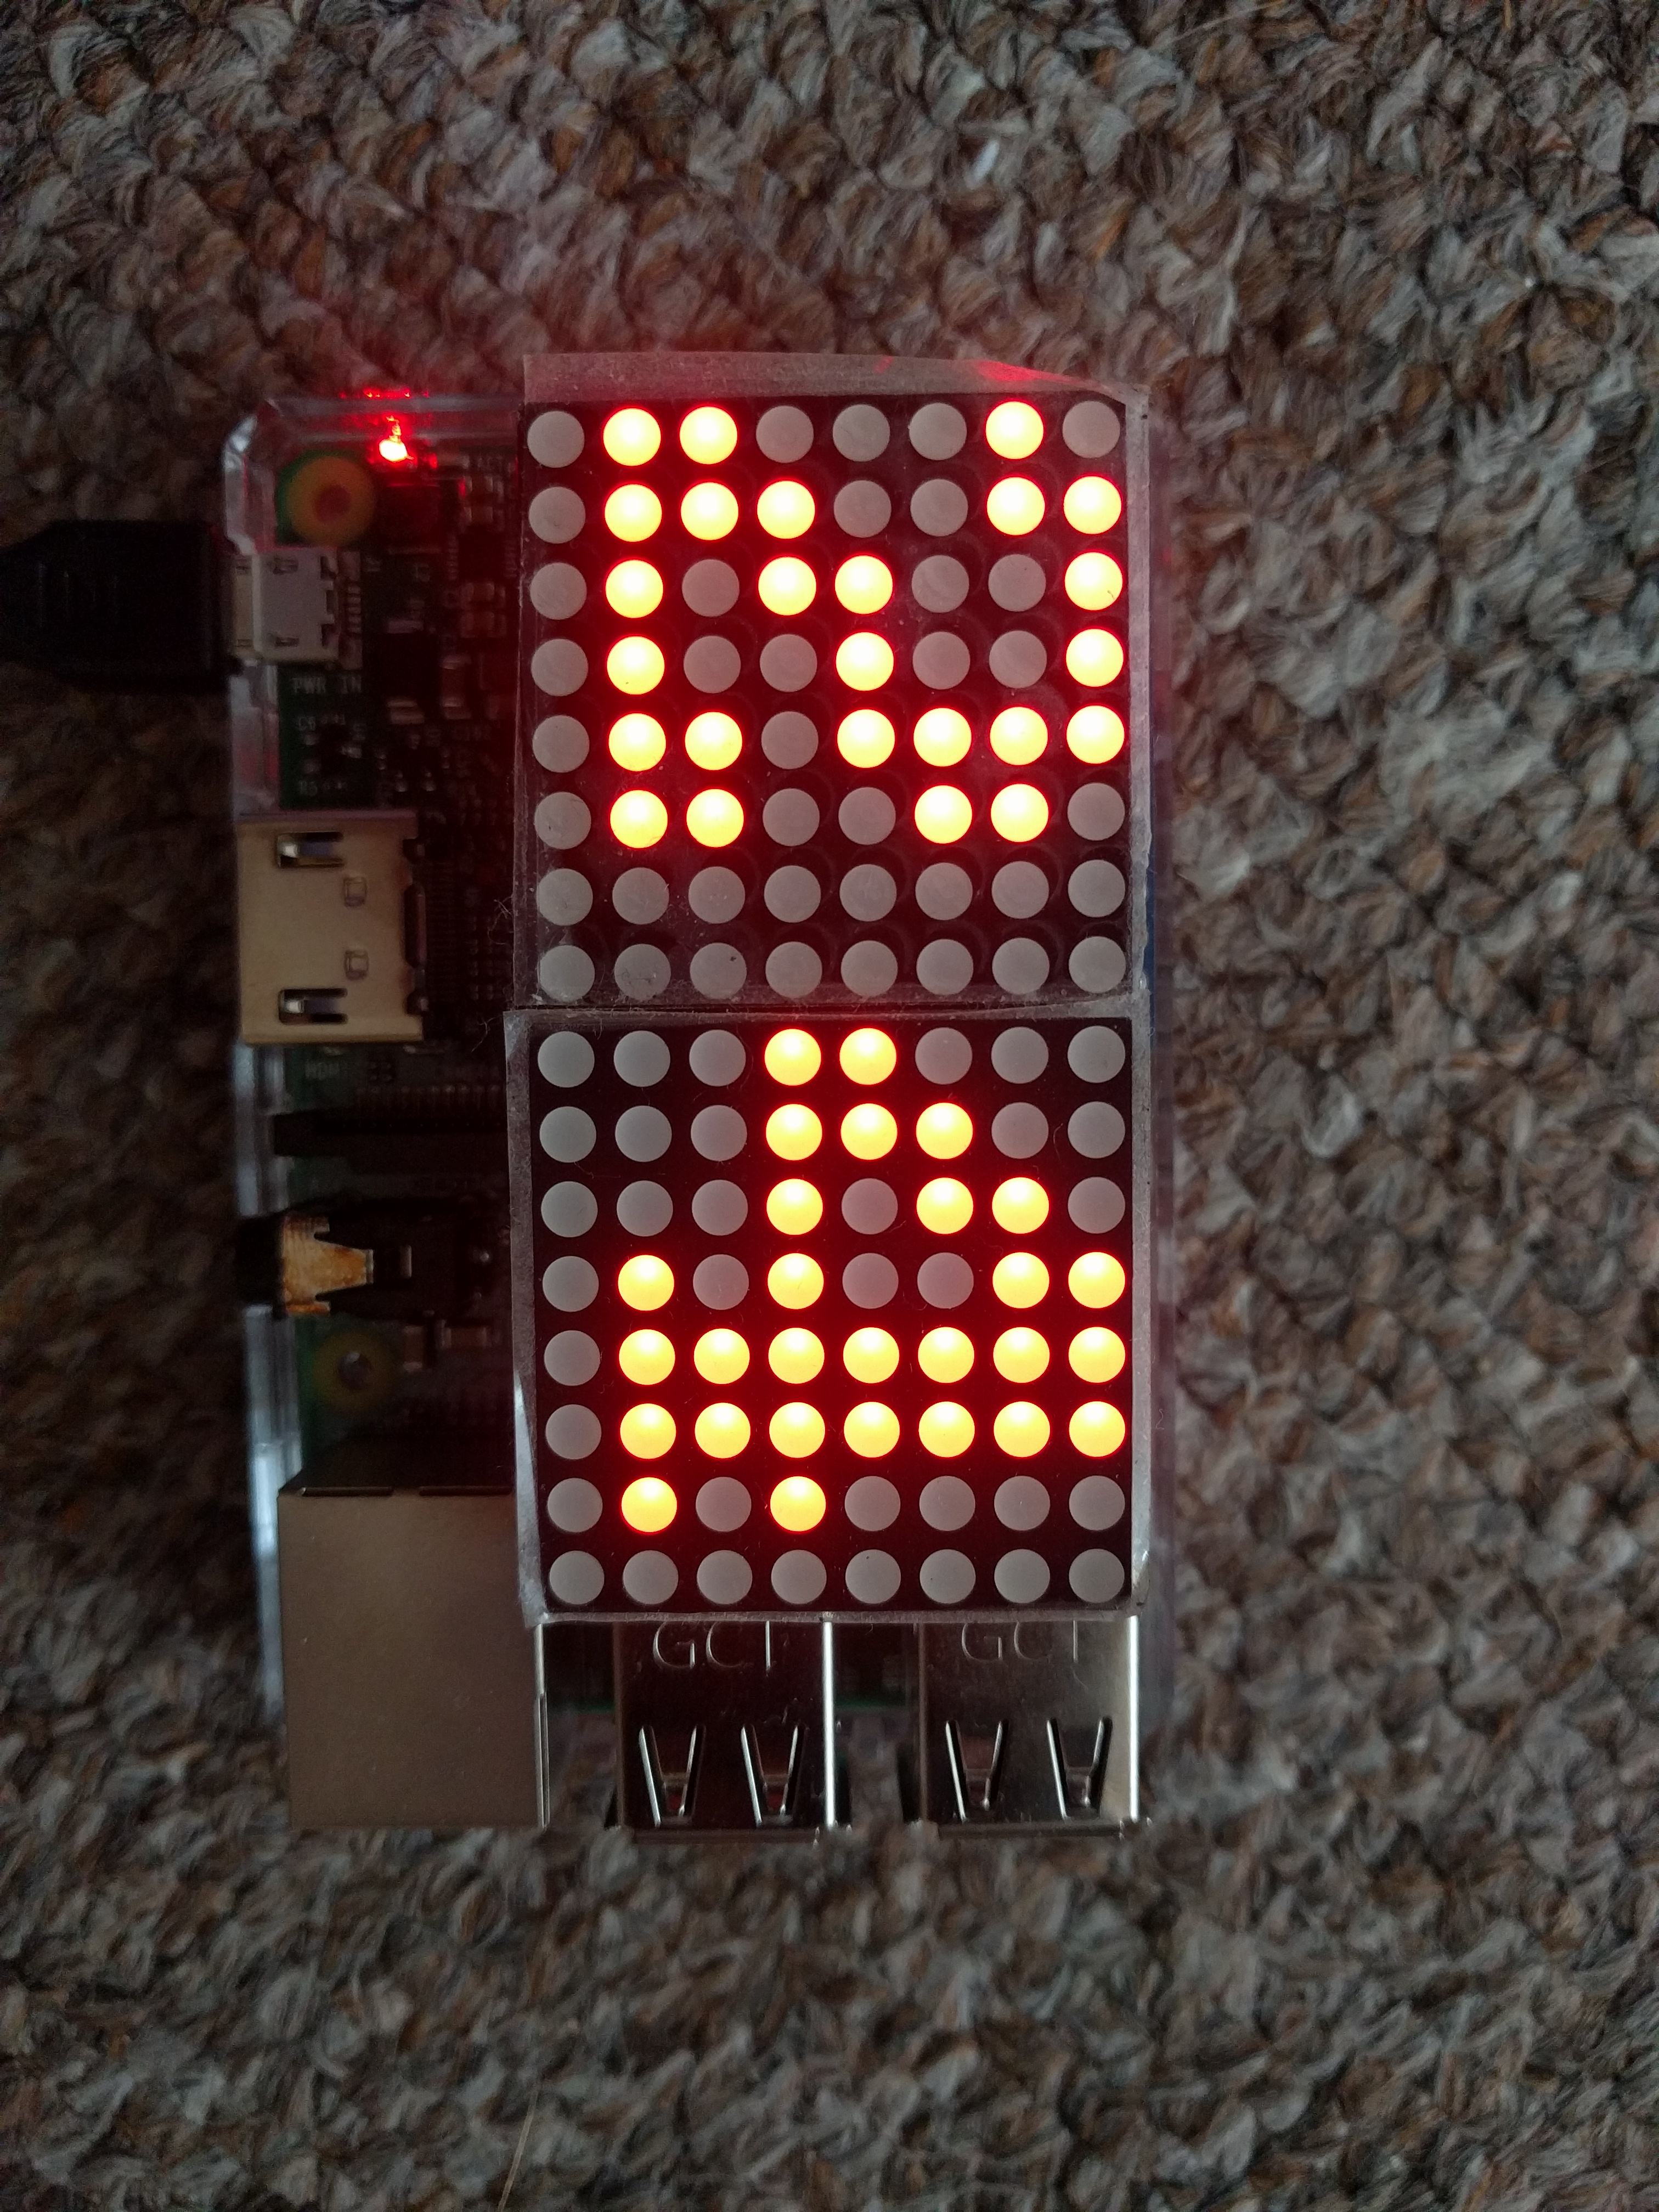
\includegraphics[angle=90,width=0.7\textwidth]{images/node.jpg}
	\caption{Zdjęcie dodatkowego węzła klastra.}
	\label{fig:led}
\end{figure}

\noindent Poniższy zrzut ekranu pokazuje natomiast wygląd aplikacji webowej \textit{KubePi Monitor}.
\begin{figure}[h]
	\centering
	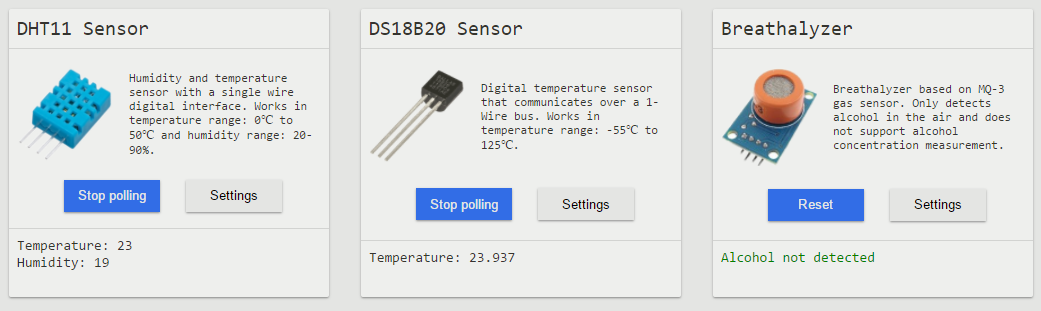
\includegraphics[width=1\textwidth]{images/kubepi-monitor.png}
	\caption{Zrzut ekranu z aplikacji KubePi Monitor.}
\end{figure}

\section{Możliwości rozszerzania projektu}
W tej części skupimy się głównie na możliwości rozwoju stworzonych aplikacji. Możemy rozważyć kilka usprawnień:

\begin{itemize}
\item{Użycie protokołu MQTT\footnote{MQTT - protokół komunikacji oparty o wzorzec subscribe/publish. Przeznaczony do transmisji danych dla urządzeń niewymagających dużej przepustowości.} zamiast architektury REST i automatyczne wysyłanie danych z czujników do centralnego serwera.}
\item{Umożliwienie dostępu do danych historycznych zebranych z czujników.}
\item{Usprawnienie aplikacji webowej poprzez umożliwienie zarządzania czujnikami wieloma jednakowymi czujnikami, np. dodanie etykiet.}
\end{itemize}
\chapter{Podsumowanie}
\section{Dyskusja wyników}
Celem pracy było stworzenie rozproszonego systemu do monitorowania otoczenia zarządzanego przez system Kubernetes, a opartego o mikrokontrolery Raspberry Pi. Głównym atutem przedstawionej architektury jest modułowa budowa oraz wysoka niezawodność. Każdy nowy węzeł może być w bardzo prosty sposób dołączony do istniejącej infrastruktury, a stworzone aplikacje szybko uruchomione. Sam system odporny jest na przerwy w zasilaniu czy błędy, ponieważ po ponownym uruchomieniu zostaje przywrócony do poprzedniego stanu.

Przedstawione aplikacje pozwalają na stworzenie prostego systemu do monitorowania naszego domu i nie tylko, a dostęp do wszelkich danych umożliwia nam aplikacja webowa. Prosta konfiguracja, niezawodność i prostota użycia to jedne z wielu zalet przedstawionego rozwiązania. To wszystko pozwala nawet mniej doświadczonym osobom na przeniesienie tej architektury i uruchomienie wszystkiego w swoim domu, a bardziej doświadczonym umożliwia rozszerzenie i dostosowanie do swoich potrzeb.

Poza działającym klastrem Raspberry Pi w pracy zebrane zostało wiele ważnych informacji z zakresu internetu rzeczy, chmur obliczeniowych, wirtualizacji oraz mikrokontrolerów. Pozwala to na łatwiejsze zrozumienie tematyki i przyswojenie wiedzy wymaganej do stworzenia takiego systemu. Dodatkowo pozwala na zapoznanie się z obsługą samych mikrokontrolerów, interfejsów komunikacyjnych, jak również procesu budowania i dystrybucji samych aplikacji.

\section{Perspektywy rozwoju pracy}
Rozważając dalszy rozwój pracy należy wziąć pod uwagę charakter całej pracy. Skupia się ona bardziej na architekturze systemu oraz zarządzaniu nim, aniżeli na projekcie samych aplikacji. W poprzednim rozdziale przedstawione zostały możliwości rozwoju samych aplikacji, warto jednak spojrzeć na całą pracę z szerszej perspektywy. Zaproponowana architektura i przedstawiona konfiguracja oferuje w zasadzie nieograniczone możliwości. Przykładowymi perspektywami rozwoju mogą być:
\begin{itemize}
\item{Rozszerzenie projektu o możliwość wykrywania i informowania użytkownika o niebezpiecznym stężeniu gazów.}
\item{Uruchomienie i rozlokowanie wielu czujników monitorujących oferujących bardziej kompleksowe monitorowanie większej powierzchni.}
\item{Stworzenie hybrydowego systemu złożonego ze standardowych komputerów oraz mikrokontrolerów. Pozwoliłoby to na wydajniejszą analizę zebranych danych.}
\item{Rozszerzenie możliwości systemu o kompleksowe zarządzania domem w oparciu o dane zebrane z czujników, np. automatycznie otwieranie/zamykanie rolet w zależności od natężenia światła.}
\end{itemize}


\addcontentsline{toc}{chapter}{Bibliografia}
\begin{thebibliography}{99}
	\bibitem{iot} {P. Raj A. C. Raman, The Internet of Things: Enabling Technologies, Platforms, and Use Cases, Auerbach Publications, 2017, ISBN: 978-1498761284}
	\bibitem{virtualization} {M. Portnoy, Virtualization Essentials, Sybex, 2016, ISBN: 978-1119267720}
	\bibitem{docker} {J. Nickoloff, Docker in Action, Manning Publications, 2016, ISBN: 978-1633430235} 
	\bibitem{webapp} {L. Shklar, R. Rosen, Web Application Architecture: Principles, Protocols and Practices, Wiley, 2009, ISBN: 978-0470518601}
	\bibitem{effectiveGo} {https://golang.org/doc/effective\_go.html - [dostęp 02.01.2017]}
	\bibitem{compileGo} {https://golang.org/cmd/compile/ - [dostęp 2.01.2017]}
	\bibitem{reactJSDoc} {https://facebook.github.io/react/docs - [dostęp 03.01.2017]}
	\bibitem{cloud} {T. Erl, R. Puttini, Z. Mahmood, Cloud Computing: Concepts, Technology \& Architecture, Prentice Hall, 2013, ISBN: 978-0133387520}
	\bibitem{kubernetes} {https://kubernetes.io/docs/home/ - [dostęp 07.01.2017]}	
	\bibitem{raspberry} {T. Short, Raspberry Pi 3: Beginner to Pro – Step by Step Guide, CreateSpace Independent Publishing Platform, 2016, ISBN: 978-1539342984}
	\bibitem{ds18b20Doc} {https://datasheets.maximintegrated.com/en/ds/DS18B20.pdf - [dostęp 11.02.2017]}
	\bibitem{max7219Doc} {https://www.sparkfun.com/datasheets/Components/General/COM-09622-MAX7219-MAX7221.pdf - [dostęp 11.02.2017]}
	\bibitem{dht11Doc} {http://www.micropik.com/PDF/dht11.pdf - [dostęp 12.02.2017]}
	\bibitem{mq3Doc} {https://www.sparkfun.com/datasheets/Sensors/MQ-3.pdf - [dostęp 12.02.2017]}
	\bibitem{cloudComputing} {https://azure.microsoft.com/pl-pl/overview/what-is-cloud-computing - [dostęp 25.02.2017]}
	\bibitem{linux} {C. Negus, Linux Bible, Wiley, 2015, ISBN: 978-1118999875}
	\bibitem{dockerhub} {https://hub.docker.com/ - [dostęp 26.02.2017]}
	\bibitem{borg} {A. Verma, L. Pedrosa, M. Korupolu, D. Oppenheimer, E. Tune, J. Wilkes, Large-scale cluster management at Google with Borg, Google Inc., 2015, https://pdos.csail.mit.edu/6.824/papers/borg.pdf - [dostęp 04.03.2017]}
	\bibitem{borgArticle} {http://itwiz.pl/borg-kubernetes-narzedzia-rozwijane-przez-google-polsce - [dostęp 04.03.2017]}
	\bibitem{raft} {https://raft.github.io - [dostęp 05.03.2017]}
	\bibitem{resin} {http://caucho.com/products/resin/doc - [dostęp 05.03.2017]}
	\bibitem{hypriotos} {https://blog.hypriot.com - [dostęp 25.03.2017]}
	\bibitem{dht11Botland} {https://botland.com.pl/czujniki-temperatury/1314-czujnik-temperatury-i-wilgotnosci-dht11.html - [dostęp 01.04.2017]}
	\bibitem{ds18b20Botland} {https://botland.com.pl/czujniki-temperatury/165-czujnik-temperatury-ds18b20-cyfrowy-1-wire-tht.html - [dostęp 01.04.2017]}
	\bibitem{max7219Botland} {https://botland.com.pl/led-do-raspberry-pi-32/4509-matryca-128-led-16x8-max7219-do-raspberry-pi.html - [dostęp 01.04.2017]}
	\bibitem{mq3Botland} {https://botland.com.pl/czujniki-gazu/5519-czujnik-alkoholu-mq-3-modul-waveshare.html - [dostęp 01.04.2017]}
	\bibitem{gorestful} {https://github.com/emicklei/go-restful - [dostęp 02.04.2017]}
	\bibitem{gorpio} {https://github.com/stianeikeland/go-rpio - [dostęp 02.04.2017]}
	\bibitem{godht} {https://github.com/d2r2/go-dht - [dostęp 02.04.2017]}
	\bibitem{gods18b20} {https://github.com/traetox/goDS18B20 - [dostęp 02.04.2017]}
	\bibitem{spidev} {https://github.com/fulr/spidev - [dostęp 02.04.2017]}	
	\bibitem{flannel} {https://github.com/coreos/flannel - [dostęp 02.04.2017]}
	\bibitem{kubepi} {https://github.com/floreks/KubePi - [dostęp 05.05.2017]}			\bibitem{xgo} {https://github.com/karalabe/xgo - [dostęp 29.04.2017]}	
	% obrazki
	\bibitem{rpiComparisonImg} {https://hackadaycom.files.wordpress.com/2016/02/pispecs2.png - [dostęp 11.02.2017]}
	\bibitem{iotImg} {https://upload.wikimedia.org/wikipedia/commons/a/ab/Internet\_of\_Things.jpg - [dostęp 07.01.2017]}
	\bibitem{cloudArchImg} {http://img.bhs4.com/89/3/893E6C660161EB50A28D2306A933F2A07F98F600\_lis.jpg - [dostęp 11.02.2017]}
	\bibitem{hypervisorArchImg} {http://www.ni.com/cms/images/devzone/tut/HostedVsBareMetal2\_20090802212753.png - [dostęp 05.05.2017]}
	\bibitem{virtContainerArchImg} {http://www.viux.com/Portals/0/images/hosting/cloud\_servers/Containers\_new\_V2.jpg - [dostęp 05.05.2017]}
	\bibitem{dockerArchImg} {https://www.sayonetech.com/media/2015/10/30/docker\_host\_image.jpg - [dostęp 05.05.2017]}
	\bibitem{borgArchImg} {https://image.slidesharecdn.com/whatdoesittaketomakegoogleworkatscale-150825083956-lva1-app6892/95/what-does-it-take-to-make-google-work-at-scale-35-638.jpg - [dostęp 05.05.2017]}
	\bibitem{kubernetesArchImg} {https://upload.wikimedia.org/wikipedia/commons/thumb/b/be/Kubernetes.png/600px-Kubernetes.png - [dostęp 05.05.2017]}
	\bibitem{dockerSwarmArchImg} {https://image.slidesharecdn.com/dockerswarmv1-150401123157-conversion-gate01/95/docker-swarm-introduction-13-638.jpg - [dostęp 05.05.2017]}
	\bibitem{rpi3Img} {https://www.raspberrypi.org/app/uploads/2016/02/Raspberry-Pi-3-top-down-web.jpg - [dostęp 05.05.2017]}
	\bibitem{pi3pinoutImg} {https://www.element14.com/community/servlet/JiveServlet/previewBody/73950-102-10-339300/pi3\_gpio.png - [dostęp 05.05.2017]}
	\bibitem{dht11Img} {https://botland.com.pl/9274-large\_default/czujnik-temperatury-i-wilgotnosci-dht11.jpg - [dostęp 05.05.2017]}
	\bibitem{ds18b20Img} {https://botland.com.pl/7798-large\_default/czujnik-temperatury-ds18b20-cyfrowy-1-wire-tht.jpg - [dostęp 05.05.2017]}
	\bibitem{max7219Img} {https://botland.com.pl/16640-large\_default/matryca-128-led-16x8-max7219-do-raspberry-pi.jpg - [dostęp 05.05.2017]}
	\bibitem{mq3Img} {https://botland.com.pl/8941-large\_default/czujnik-alkoholu-mq-3.jpg - [dostęp 05.05.2017]}
	\bibitem{hypriot} {https://blog.hypriot.com/downloads/ - [dostęp 05.05.2017]}
	\bibitem{etcher} {https://blog.hypriot.com/downloads/ - [dostęp 05.05.2017]}
\end{thebibliography}

\addcontentsline{toc}{chapter}{Spis rysunków}
\listoffigures

\end{document}
